\documentclass[cjk,slidestop,compress,mathserif,blue]{beamer}
%dvipdfm选项是关键,否则编译统统通不过
%beamer的颜色选项定义的是导航条和标题的颜色(即关键词structure的颜色)

%%%%%%%%%%%%%%%%仅限于XeTeX可使用的宏包%%%%%%%%%%%%%%%%%%%%%%%%%%%%
\usepackage{fontspec,xunicode,xltxtra,beamerthemesplit}
%\usepackage{beamerthemesplit}
\usepackage{xeCJK}
\setCJKmainfont[BoldFont=黑体, ItalicFont=楷体, BoldItalicFont=仿宋]{黑体}
%\setsansfont[Mapping=tex-text]{Adobe 黑体 Std}
%如果装了Adobe Acrobat,可在font.conf中配置Adobe字体的路径以使用其中文字体
%也可直接使用系统中的中文字体如SimSun,SimHei,微软雅黑 等
%原来beamer用的字体是sans family;注意Mapping的大小写,不能写错

%%%%%%%%   确定标题和导航条结构的框架     %%%%%%%%%%%%
\usepackage{beamerthemeshadow}                       %
%\usepackage{beamerthemeclassic}%导航条色与背景色一致%
%%%%%%%%%%%%%%%%%%%%%%%%%%%%%%%%%%%%%%%%%%%%%%%%%%%%%%
\setbeamerfont{roman title}{size={}}
%\usepackage{CJK} % CJK 中文支持                                  %
\usepackage{amsmath,amsthm,amsfonts,amssymb,bm}
\usepackage{mathrsfs}
\usepackage{xcolor}                                        %使用默认允许使用颜色
\usepackage{enumerate}                                     %使用标注数字
\usepackage{hyperref} 
\usepackage{graphicx}
\usepackage{subfigure}           %图片跨页

%\usepackage[numbers,sort&compress]{natbib} %紧密排列             %
\usepackage[sectionbib]{chapterbib}        %每章节单独参考文献   %
\usepackage{hypernat}                                                                         %
%\usepackage[dvipdfm,bookmarksopen=true,pdfstartview=FitH,CJKbookmarks]{hyperref}		%
\hypersetup{bookmarksnumbered,colorlinks,linkcolor=brown,citecolor=blue,urlcolor=red}         %
%参考文献含有超链接引用时需要下列宏包,注意与natbib有冲突        %
%\usepackage[dvipdfm]{hyperref}                                  %
%\usepackage{hypernat}                                           %
\newcommand{\upcite}[1]{\hspace{0ex}\textsuperscript{\cite{#1}}} %

%\useoutertheme{smoothbars}
\useinnertheme[shadow=true]{rounded}
\usetheme{Berkeley}                                          %主题式样
%\usetheme{Luebeck}

\usecolortheme{lily}                                        %颜色主题式样

\usefonttheme{professionalfonts}                           %字体主题样式宏包

%\beamertemplatetransparentcoveredhigh                      %使所有被隐藏的文本高度透明
\beamertemplatetransparentcovereddynamicmedium             %使所有被隐藏的文本完全透明,动态,动态的范围很小
\mode<presentation>
%\beamersetaveragebackground{gray}                          %设置背景颜色(单一色) 
\beamertemplateshadingbackground{green!10}{red!5}         %设置背景颜色(渐变色)

%i放置单位logo
%\logo{
\includegraphics[width=1.6cm,height=0.35cm]{Figures/BCC_logo-1.png}}	%简单设置logo

%\pgfdeclareimage[width=3.5cm]{logoname}{Figures/BCC_logo-1.png}		%logo置于左侧微调
%\logo{\pgfuseimage{logoname}{\vspace{0.2cm}\hspace*{-2.0cm}}}

%在指定位置精确放置logo
\usepackage{tikz}
\usepackage{beamerfoils}
\usepackage{pgf}
\logo{\pgfputat{\pgfxy(11.68,0.15)}{
\includegraphics[height=1.01cm,viewport=0 0 140 120,clip]{Figures/BCC_logo-1.png}}\pgfputat{\pgfxy(10.502,-0.218)}{
\includegraphics[height=0.369cm,viewport=140 0 540 120,clip]{Figures/BCC_logo-1.png}}}
%\logo{\pgfputat{\pgfxy(11.68,0.15)}{
\includegraphics[height=0.95cm,viewport=0 0 510 360,clip]{Figures/Logo_Gainstrong.png}}\pgfputat{\pgfxy(10.333,-0.195)}{
\includegraphics[height=0.35cm,viewport=530 70 1100 218,clip]{Figures/Logo_Gainstrong.png}}}
%\MyLogo{
%	\pgfputat{\pgfxy(-50,-50)}{\pgfbox[right,base]{
\includegraphics[height=1cm]{Figures/BCC_logo-1.png}}}

%logo作为背景放置
%\setbeamertemplate{background}{
%	\pgfputat{\pgfxy(6.5,-0.5)}{\pgfbox[left,top]{\pgfimage[height=1.1cm]{Figures/BCC_logo-1.png}}}}

%\logo{}									%不显示logo

\begin{document}
%\begin{CJK*}{GBK}{song}
%\begin{CJK*}{GBK}{kai}
%beamer下不能用\songyi、\zihao等命令!
%\graphicspath{Figures/}

%-------------------------------PPT Title-------------------------------------
\title{线性响应理论与光学函数}
%-----------------------------------------------------------------------------

%----------------------------Author & Date------------------------------------
\author{北京市计算中心\;云平台\:姜骏}
\date{\textrm{2016.11.23}}
%\date{2013.09.10}
\frame{\titlepage}
%-----------------------------------------------------------------------------

%------------------------------------------------------------------------------列出全文 outline ---------------------------------------------------------------------------------
\section*{}
\frame[allowframebreaks]
{
  \frametitle{Outline}
%  \frametitle{\textcolor{mycolor}{\secname}}
  \tableofcontents%[current,currentsection,currentsubsection]
}
%在每个section之前列出全部Outline
%类似的在每个subsection之前列出全部Outline是\AtBeginSubsection[]
\AtBeginSection[]
{
  \frame<handout:0>
  {
    \frametitle{Outline}
%全部Outline中,本部分加亮
    \tableofcontents[current,currentsection]
  }
}

%------------------------------------------------------------------------------PPT main Body------------------------------------------------------------------------------------
\small
\section{线性响应理论}
\frame
{
	\frametitle{线性响应与响应函数}
	\begin{itemize}
		\item 对系统施加外场(某种扰动),系统的某些物理性质会产生相应的变化称为\textcolor{red}{响应}(\textrm{response})
		\item \textcolor{red}{线性响应}:~如果外场(扰动)较小,物理量的变化(响应)与施加的外场成正比,即线性关系\\
			线性系数一般称为\textcolor{blue}{线性响应函数}(\textrm{linear response function})
		\item 线性响应的条件
			\begin{description}
				\item[1] 扰动较小,可作微扰处理
				\item[2] 物理量的响应能及时追随扰动
			\end{description}
		\item \textcolor{blue}{线性响应理论应用}
			\begin{itemize}
				\item 平衡几何构型与晶格振动:~晶格动力学
				\item 电场响应函数:~电子激发与介电函数
				\item 自旋响应函数:~磁振子
			\end{itemize}
	\end{itemize}
}

\frame
{
	\frametitle{简谐近似}
	\begin{itemize}
		\item 晶体中的格点表示原子的平衡位置,晶格振动是原子在格点附近的振动
		\item 红外、Raman光谱、中子衍射谱,热容、热导,电阻、超导和电-声耦合等都与晶格振动有关
		\item 绝热近似(\textrm{Born-Oppenheimer}近似)下,原子核是在电子总能量$E(\mathbf{R})$形成的势能面上运动
	\end{itemize}
	含有$N$个原子,平衡位置是$\mathbf{R}_i^0$,偏移位置矢量$\mathbf{\mu}_i(t)$,体系的势能函数在平衡位置作\textrm{Taylor~}级数展开
	\begin{displaymath}
%		\begin{aligned}
		V=V_0+\sum_{i=1}^{3N}\left( \frac{\partial V}{\partial \mu_i} \right)_0\mu_i+\underline{\textcolor{red}{\frac12\sum_{i,j=1}^{3N}\left( \frac{\partial^2V}{\partial\mu_i\partial\mu_j} \right)_0\mu_i\mu_j}}+\mbox{高阶项}
%		\end{aligned}
	\end{displaymath}
	平衡位置$\left( \frac{\partial V}{\partial\mu_i} \right)_0=0$,\textcolor{blue}{简谐近似}保留到$\mu_i$的二次项
}

\frame
{
	\frametitle{简正坐标与简谐振动}
	$N$原子体系的动能函数
	\begin{displaymath}
		T=\frac12\sum_{i=1}^{3N}m_i\dot{\mu}_i^2
	\end{displaymath}
	引入简正坐标,\textcolor{blue}{与原子位移坐标$\mu_i$正交变换}
	\begin{displaymath}
		\sqrt{m_i}\mu_i=\sum_{j=1}^{3N}a_{ij}Q_j
	\end{displaymath}
	\textcolor{red}{目的}:~系统的势能函数与动能函数有简单形式(只有平方项)
	\begin{displaymath}
%		\begin{aligned}
			T=\frac12\sum_{i=1}^{3N}\dot{Q}_i^2\quad
			V=\frac12\sum_{i=1}^{3N}\omega_i^2Q_i^2
%		\end{aligned}
	\end{displaymath}
	由此可得谐振方程
	\begin{displaymath}
		\ddot{Q}_i+\omega_i^2Q_i=0\quad i=1,2,3,\cdots,3N
	\end{displaymath}

}

\frame
{
	\frametitle{简谐振动与振动模式}
	任意简正坐标解
	\begin{displaymath}
		Q_i=A\sin(\omega_it+\delta)
	\end{displaymath}
	由此得到原子位移坐标
	\begin{displaymath}
		\mu_i=\frac{a_{ij}}{\sqrt{m_i}}A\sin(\omega_it+\delta)
	\end{displaymath}
\begin{figure}[h!]
\centering
%\hspace*{-10pt}
\vspace*{-0.1in}
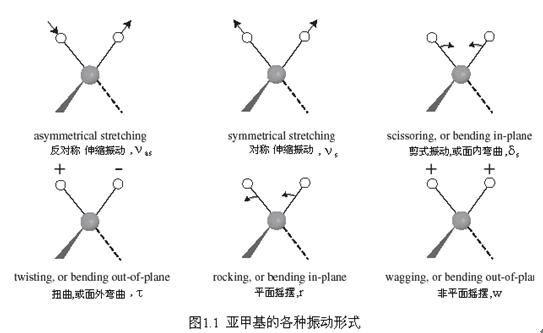
\includegraphics[height=1.in,width=2.in,viewport=0 20 420 250,clip]{Figures/RF_vir.jpg}
\caption{\small \textrm{Schematic example of vibration model of dimethyl.}}%
\label{virbration_model}
\end{figure} 
\textcolor{red}{简谐振动不表示某个原子的振动,表示整个体系所有原子参与的振动。这种体系中所有原子一起参加的共同振动常称为振动模}
}

\frame
{
	\frametitle{一维单原子链}
\begin{figure}[h!]
\centering
%\hspace*{-10pt}
\vspace*{-0.25in}
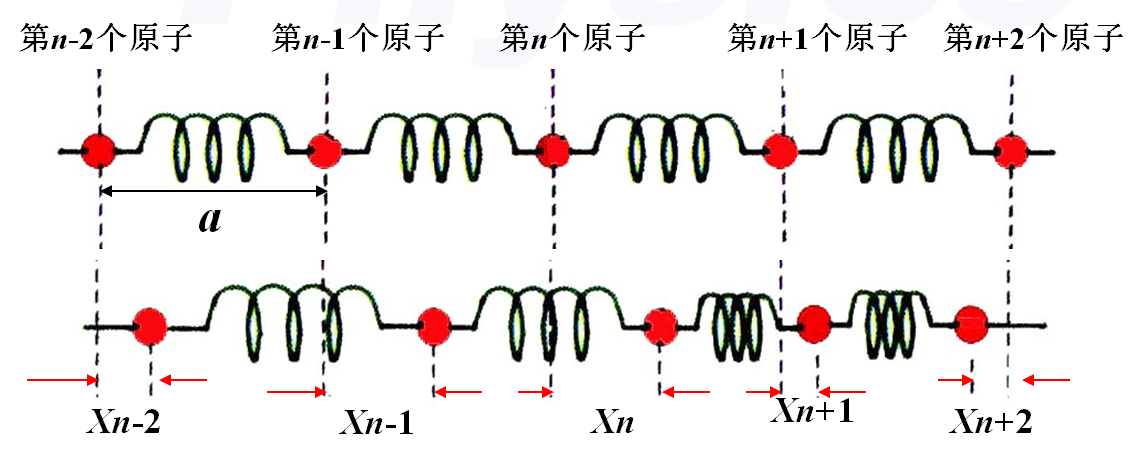
\includegraphics[height=1.0in,width=2.8in,viewport=0 0 1400 500,clip]{Figures/virbration.png}
\caption{\small \textrm{Schematic example of vibration of 1D-atomic chain.}}%
\label{virbration}
\end{figure} 
单原子链可以视为最简单的晶格,平衡时相邻原子距离为$\mathbf{a}$,原子限制在沿链方向运动,偏离格点位置用$\cdots,\mathbf{X}_{n-1},\mathbf{X}_{n},\mathbf{X}_{n+1},\cdots$,原子的振动可以表示为
\begin{displaymath}
	\mu_{nq}=A\mathrm{e}^{\mathrm{i}(\omega t-qx)}
\end{displaymath}
其中振幅$A$是常数,$\omega$是圆频率,$q=\tfrac{2\pi}{\lambda}$是波数,$\lambda$是波长\\
\textcolor{blue}{根据量子理论,每种简谐振动的能量是量子化的,可以用声子表示}
\begin{displaymath}
	\varepsilon_{nq}=\left( n+\frac12 \right)\hbar\omega_q
\end{displaymath}
}

\frame
{
	\frametitle{双原子链与光学支和声学支}
\begin{figure}[h!]
\centering
%\hspace*{-10pt}
\vspace*{-0.25in}
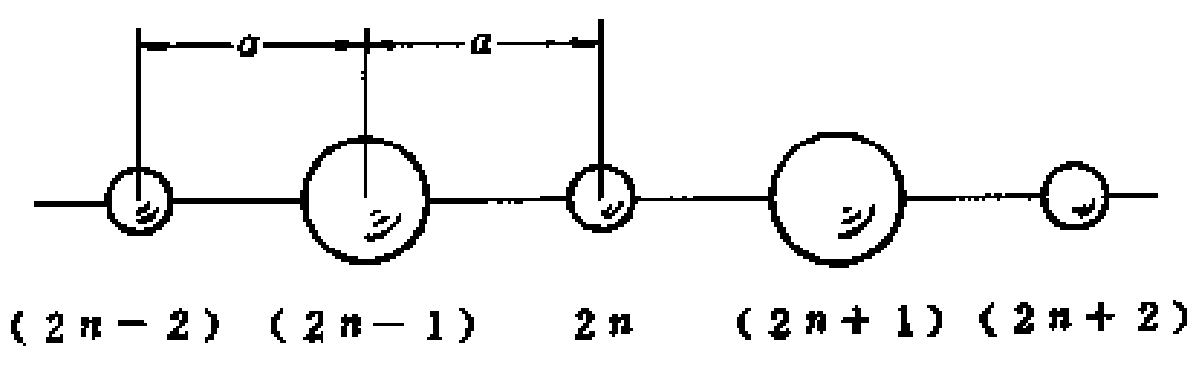
\includegraphics[height=0.7in,width=2.6in,viewport=0 0 1400 400,clip]{Figures/virbration-2.png}
\caption{\small \textrm{Schematic example of vibration of 1D-diatomic chain.}}%
\label{virbration-2D}
\end{figure} 
一维双原子链是最简单的复式晶格,平衡时相邻原子间距为$\mathbf{a}$,每个原胞含有两个不同原子\textrm{P}和\textrm{Q}质量分别是$m$和$M$,原子现在在沿链方向运动,偏离位移用$\cdots,\mu_{2n},\mu_{2n+1},\cdots$\\原子的运动方程
\begin{displaymath}
	\begin{aligned}
		&\mbox{\textrm{P}原子:~}m\ddot{\mu}_{2n}=-\beta(2\mu_{2n}-\mu_{2n+1}-\mu_{2n-1})\\
		&\mbox{\textrm{Q}原子:~}M\ddot{\mu}_{2n+1}=-\beta(2\mu_{2n+1}-\mu_{2n+2}-\mu_{2n})
	\end{aligned}
\end{displaymath}
可得关于振动频率$\omega$的两组解
\begin{displaymath}
	\omega^2\left.
	\begin{aligned}
		&\nearrow\omega_+^2\\
		&\searrow\omega_-^2
	\end{aligned}\right\}
	=\beta\frac{m+M}{mM}\left\{ 1\pm\left[ 1-\frac{4mM}{(m+M)^2}\sin^2aq \right]^{1/2} \right\}
\end{displaymath}
}

\frame
{
	\frametitle{光学支和声学支的长波极限}
\begin{figure}[h!]
\begin{minipage}[t]{0.3\linewidth}
\centering
\vspace*{-0.3in}
%\hspace*{-10pt}
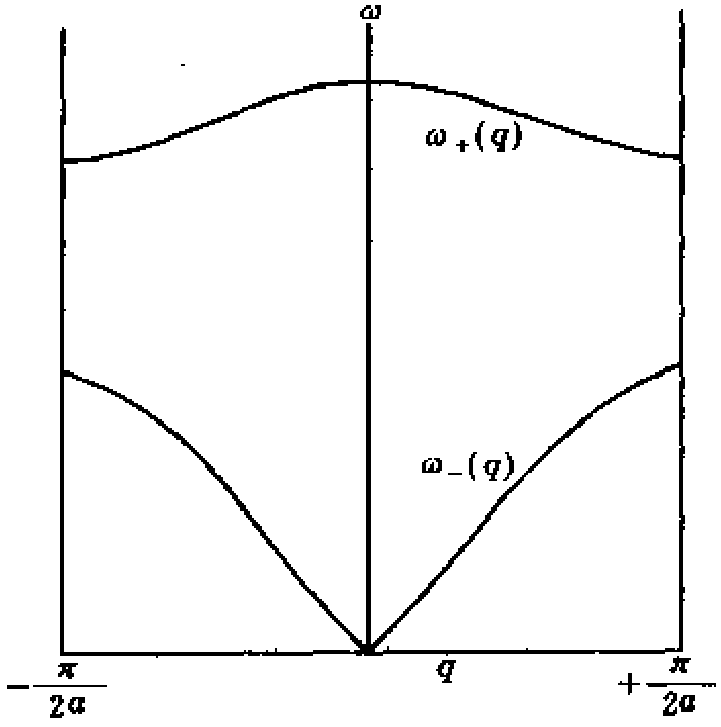
\includegraphics[height=1.in,width=1.in,viewport=0 0 700 800,clip]{Figures/Optic-Acous.png}
\label{optic_acous}
\end{minipage}
\hfill
\begin{minipage}[t]{0.67\linewidth}
%\vspace*{-0.3in}
	\begin{itemize}
		\item \textcolor{blue}{光学支}:~属于频率$\omega_+$的晶格简谐振动
		\item \textcolor{blue}{声学支}:~属于频率$\omega_-$的晶格简谐振动
	\end{itemize}
\end{minipage}
\caption{\small \textrm{The acoustic branch and optical branch.}}%
\end{figure} 
声学支的长波极限($q\rightarrow0$):
\begin{displaymath}
	\omega_-\approx a\sqrt{\frac{2\beta}{m+M}}q\quad\mbox{\textcolor{blue}{一维链看成连续介质的弹性波}}
\end{displaymath}
光学支的长波极限($q\rightarrow0$):
\begin{displaymath}
	\omega_+\approx a\sqrt{\frac{2\beta}{\left( \frac{mM}{m+M} \right)}}\quad\mbox{\textcolor{blue}{两种原子具有相反的相位,质心保持不动}}
\end{displaymath}
}

\frame
{
	\frametitle{经典三维振动模式}
			位于$\mathbf{R}_I(t)$的原子核运动的经典力学描述
			\begin{displaymath}
				M_I\frac{\partial^2\mathbf{R}_I}{\partial t^2}=\vec F_I(\mathbf{R})=-\frac{\partial}{\partial\mathbf{R}_I}E(\mathbf{R})
			\end{displaymath}
			晶格平衡位置$\{\mathbf{R}_I^0\}=\mathbf R^0$由原子核受力平衡确定
			\begin{displaymath}
				\vec F_I(\mathbf R^0)=0
			\end{displaymath}
			\textcolor{blue}{对平衡位置偏移的受力方程为}
			\begin{displaymath}
				C_{I,\alpha;J,\beta}=\frac{\partial^2E(\mathbf{R})}{\partial\mathbf{R}_{I,\alpha}\partial\mathbf{R}_{J,\beta}}
			\end{displaymath}
			其中$\alpha,\beta\cdots$是\textrm{cartesian}坐标

			\textcolor{blue}{谐振子近似下},频率为$\omega$的谐振模式下,晶格对平移位置的偏移为
			\begin{displaymath}
				\mathbf{u}_I(t)=\mathbf{R}_I(t)-\mathbf{R}_I^0\equiv\mathbf{u}_I\mathrm{e}^{\mathrm{i}\omega t}
			\end{displaymath}
			对位于$I$的原子核(质量为$M_I$),有
			\begin{displaymath}
				-\omega^2M_Iu_{I\alpha}=-\sum_{J\beta}C_{I,\alpha;J\beta}u_{J\beta}
			\end{displaymath}
			因此振动频率$\omega$,由经典谐振方程确定
			\begin{displaymath}
				\det\left|\frac1{\sqrt{M_IM_J}}C_{I,\alpha;J\beta}-\omega^2\right|=0
			\end{displaymath}
}

\frame
{
	\frametitle{晶格振动模式(冻声子方法)}
	对于周期性的晶格振动,根据\textrm{Bl\"och~}定理,振动引起的位置偏移
			\begin{displaymath}
				\mathbf{u}_s(\vec T_n)\equiv\mathbf{R}_s(\vec T_n)-\mathbf{R}_s^0(\vec T_n)=\mathrm{e}^{\mathrm{i}\vec k\cdot\vec T_n}\mathbf{u}_s(\vec k)
			\end{displaymath}
			由此得谐振方程
			\begin{displaymath}
				\det\left|\frac1{\sqrt{M_sM_{s^{\prime}}}}C_{s,\alpha;s^{\prime}\alpha^{\prime}}-\omega_{i\vec k}^2\right|=0
			\end{displaymath}
			这里原子标记$s=1,S$,对应的谐振模式$i=1,3S$

			每个$\vec k$的约化力常数矩阵可表示为
			\begin{displaymath}
				\begin{aligned}
				C_{s,\alpha;s^{\prime}\alpha^{\prime}}(\vec k)=&\sum_{\vec T_n}\mathrm{e}^{\mathrm{i}\vec k\cdot\vec T_n}\frac{\partial^2 E(\mathbf{R})}{\partial\mathbf{R}_{s,\alpha}(0)\partial\mathbf{R}_{s^{\prime},\alpha^{\prime}}(\vec T_n)}\\
				=&\frac{\partial^2E(\mathbf{R})}{\partial\mathbf{u}_{s,\alpha}(\vec k)\partial\mathbf{u}_{s^{\prime},\alpha^{\prime}}(\vec k)} 
				\end{aligned}
			\end{displaymath}
}

\frame
{
	\frametitle{声子与密度响应函数}
	谐振的力常数是能量的两阶导数,因此最初由响应函数计算声子时,即采用两阶微扰理论

	对于随参数$\lambda_i$变化的外势$V_{ext}(\vec r)$的响应中包含一般表达式
	\begin{displaymath}
		\begin{aligned}
			\frac{\partial E}{\partial\lambda_i}=&\frac{\partial E_{\mathrm{ion}}}{\partial\lambda_i}+\int\frac{\partial V_{ext}(\vec r)}{\partial\lambda_i}n(\vec r)\mathrm{d}\vec r\quad\mbox{\textcolor{red}{即\textrm{Hellmann-Feynman}力}}\\
			\frac{\partial^2E}{\partial\lambda_i\partial\lambda_j}=&\frac{\partial^2E_{\mathrm{ion}}}{\partial\lambda_i\partial\lambda_j}+\int\frac{\partial^2V_{ext}(\vec r)}{\partial\lambda_i\partial\lambda_j}n(\vec r)\mathrm{d}\vec r+\underline{\int\frac{\partial n(\vec r)}{\partial\lambda_i}\frac{\partial V_{ext}(\vec r)}{\partial\lambda_j}\mathrm{d}\vec r}
		\end{aligned}
	\end{displaymath}
	其中
	\begin{displaymath}
		\begin{aligned}
	\int\frac{\partial n(\vec r)}{\partial\lambda_i}\frac{\partial V_{ext}(\vec r)}{\partial\lambda_j}\mathrm{d}\vec r=&\int\frac{\partial V_{ext}(\vec r^{\prime})}{\partial\lambda_i}\frac{\partial n(\vec r)}{\partial V_{ext}(\vec r^{\prime})}\frac{\partial V_{ext}(\vec r)}{\partial\lambda_j}\mathrm{d}\vec r\mathrm{d}\vec r^{\prime}\\
		=&\int\frac{\partial V_{ext}(\vec r^{\prime})}{\partial\lambda_i}\chi(\vec r,\vec r^{\prime})\frac{\partial V_{ext}(\vec r)}{\partial\lambda_j}\mathrm{d}\vec r\mathrm{d}\vec r^{\prime}
		\end{aligned}
	\end{displaymath}
	这里\textcolor{red}{$\chi$是密度响应函数}
}

\frame
{
	\frametitle{密度响应函数与\textrm{Green's function}表示}
	密度响应函数$\chi$可以在$\vec r$空间或$\vec q$空间表示
	\begin{displaymath}
		\chi(\vec r,\vec r^{\prime})=\frac{\delta n(\vec r)}{\delta V_{ext}(\vec r^{\prime})}\qquad\chi(\vec q,\vec q^{\prime})=\frac{\delta n(\vec q)}{\delta V_{ext}(\vec q^{\prime})}
	\end{displaymath}
	响应函数可表示为
	\begin{displaymath}
		\chi=\frac{\delta n}{\delta V_{\mathrm{eff}}}\frac{\delta V_{\mathrm{eff}}}{\delta V_{ext}}=\chi^0\left[1+\frac{\delta V_{int}}{\delta n}\frac{\delta n}{\delta V_{ext}}\right]=\chi^0[1+K\chi]
	\end{displaymath}
	其中$\chi^0$是无相互作用的响应函数,$K$是\textrm{kernel~}函数
	\begin{displaymath}
		\chi_n^0(\vec r,\vec r^{\prime})=\frac{\delta n(\vec r)}{\delta V_{\mathrm{eff}}(\vec r^{\prime})}=2\sum_{i=1}^{\mathrm{occ}}\sum_j^{\mathrm{empty}}\frac{\psi_i^{\ast}(\vec r)\psi_j(\vec r)\psi_j^{\ast}(\vec r^{\prime})\psi_i(\vec r^{\prime})}{\varepsilon_i-\varepsilon_j}
	\end{displaymath}
	可用\textrm{Green's function}表示
	\begin{displaymath}
		\chi_n^0(\vec r,\vec r^{\prime})=\sum_{i=1}^{\mathrm{occ}}\psi_i^{\ast}(\vec r)G_0^i(\vec r,\vec r^{\prime})\psi_i(\vec r^{\prime})\qquad G_0^i(\vec r,\vec r^{\prime})=\sum_{j\neq i}^{\infty}\frac{\psi_j(\vec r)\psi_j^{\ast}(\vec r^{\prime})}{\varepsilon_i-\varepsilon_j}
	\end{displaymath}
}

\frame
{
	\frametitle{密度响应函数的$\vec q$空间表示}
	注意到$\vec r$空间电荷密度变化
	\begin{displaymath}
		\Delta n(\vec r)=\sum_{i=1}^{\mathrm{occ}}\sum_j^{\mathrm{empty}}\psi_i^{\ast}(\vec r)\psi_j(\vec r)\frac{\langle\psi_j|\Delta V_{\mathrm{eff}}|\psi_i\rangle}{\varepsilon_i-\varepsilon_j}+\mathrm{c.c.}
	\end{displaymath}
	因此在$\vec q$空间表示中,$\Delta V_{\mathrm{eff}}(\vec r)=\Delta V_{\mathrm{eff}}\mathrm{e}^{\mathrm{i}\vec q\cdot\vec r}$,$n(\vec q^{\prime})=\int\mathrm{d}\vec rn(\vec r)\mathrm{e}^{\mathrm{i}\vec q\cdot\vec r}$,\\可有
	\begin{displaymath}
		\chi_n^0(\vec q,\vec q^{\prime})=\frac{\delta n(\vec q^{\prime})}{\delta V_{\mathrm{eff}}(\vec q)}=2\sum_{i=1}^{\mathrm{occ}}\sum_j^{\mathrm{empty}}\frac{M_{ij}^{\ast}(\vec q)M_{ij}(\vec q^{\prime})}{\varepsilon_i-\varepsilon_j}
	\end{displaymath}
	这里$M_{ij}(\vec q)=\langle\psi_i|\mathrm{e}^{\mathrm{i}\vec q\cdot\vec r}|\psi_j\rangle$\\
	\vspace{10pt}
	\textcolor{blue}{显然对于周期体系,$\chi_n^0$在$\vec q$空间表示更方便}
	
	对于均匀电子气,只有$\vec q=\vec q^{\prime}$,$\chi_n^0(\vec q,\vec q^{\prime})\neq0$
}

\frame
{
	\frametitle{密度响应函数与声子}
	\textrm{kernel~}函数$K$的表达式
	\begin{displaymath}
		K(\vec q,\vec q^{\prime})=\frac{\delta V_{ini}(\vec q)}{\delta n(\vec q^{\prime})}=\frac{4\pi}{q^2}\delta_{\vec q,\vec q^{\prime}}+\frac{\delta^2 E_{\mathrm{XC}}[n]}{\delta n(\vec q)\delta n(\vec q^{\prime})}\equiv V_C(q)\delta_{\vec q,\vec q^{\prime}}+f_{\mathrm{XC}}(\vec q,\vec q^{\prime})
	\end{displaymath}
	\textcolor{red}{注意}:~当$f_\mathrm{XC}=0$即无规相近似(\textrm{random phase approximation, RPA})\\
	由此可得
	\begin{displaymath}
		\chi=\chi^0[1-\chi^0K]^{-1}\qquad\chi^{-1}=[\chi^0]^{-1}-K
	\end{displaymath}
介电函数也可以用响应函数表示
	\begin{displaymath}
		\epsilon^{-1}=1+V_\mathrm{C}\chi
	\end{displaymath}
	因此对于\textit{sp}-型金属,$\chi$可以用均匀电子气模型表示(\textrm{Lindhard}介电函数$\epsilon^{-1}(|\vec q|)$),但是对于一般材料介电函数$\epsilon^{-1}(\vec q,\vec q^{\prime})$变成很大的矩阵$\epsilon_{\vec G\vec G^{\prime}}^{-1}(\vec k)$,计算非常困难
}

\frame
{
	\frametitle{\textrm{Green's function~}方法}
	\begin{itemize}
		\item 利用标准微扰理论,计算介电函数矩阵倒数$\epsilon_{\vec G\vec G^{\prime}}^{-1}(\vec k)$虽然\textcolor{blue}{能给出全部可能微扰的响应},但涉及\textcolor{red}{对全部未占据态的求和},计算效率很低
		\item 近年来发展的密度泛函微扰理论\textrm{(density functional perturbation theory, DFPT)}只关注\textcolor{blue}{特定微扰的响应},因此\textcolor{red}{计算中只需要对占据态的求和},大大提高计算效率
			\begin{enumerate}
				\item 响应函数的自洽方程用波函数改变表示\\
					电荷密度的一阶改变
					\begin{displaymath}
						\Delta n(\vec r)=2\mathrm{Re}\sum_{\i=1}^N\psi_i(\vec r)\Delta\psi_i(\vec r)
					\end{displaymath}
					其中$\Delta\psi_i(\vec r)$由一阶微扰计算
					\begin{displaymath}
						(H_{\mathrm{KS}}-\varepsilon_i)|\Delta\psi_i\rangle=-(\Delta V_{\mathrm{KS}}-\Delta\varepsilon_i)|\psi_i\rangle
					\end{displaymath}
			\end{enumerate}
	\end{itemize}
}

\frame
{
	\frametitle{\textrm{Green's function~}方法}
	$\Delta\varepsilon_i=\langle\psi_i|\Delta V_{\mathrm{KS}}|\psi_i\rangle$,因此有效势的改变可用电荷密度的变化表示
	\begin{displaymath}
		\begin{aligned}
			\Delta V_{\mathrm{KS}}(\vec r)=&\Delta V_{ext}(\vec r)+e^2\int\mathrm{d}\vec r^{\prime}\frac{\Delta n(\vec r^{\prime})}{|\vec r-\vec r^{\prime}|}+\int\mathrm{d}\vec r^{\prime}\frac{\mathrm{d}V_{\mathrm{XC}}(\vec r)}{\mathrm{d}n(\vec r^{\prime})}\Delta n(\vec r^{\prime})\\
			\equiv&\Delta V_{ext}(\vec r)+\int\mathrm{d}r^{\prime}K(\vec r,\vec r^{\prime})\Delta n(\vec r)
		\end{aligned}
	\end{displaymath}
	根据\textrm{kernel~}函数的定义,其中交换-相关部分贡献的一阶近似为$f_{\mathrm{XC}}(\vec r,\vec r^{\prime})=\tfrac{\mathrm{d}V_{\mathrm{XC}}(\vec r)}{\mathrm{d}n(\vec r^{\prime})}$
	\begin{itemize}
		\item \textcolor{blue}{根据标准微扰理论,由于电荷密度的变化遍及全部占据态($i\leqslant N$)和未占据态($j>N$)求和,因此计算效率不高}
		\item \textcolor{red}{更有效的办法是将密度和有效势的变化$\Delta n$、$\Delta V_{\mathrm{KS}}$看做为外势变化$\Delta V_{ext}$的自洽响应}\\
定义投影算符
\begin{displaymath}
%	\begin{aligned}
		\hat P_{\mathrm{occ}}=\sum_{i=1}^N|\psi_i\rangle\langle\psi_i|\quad\mbox{(占据态)}\quad%\\
		\hat P_{\mathrm{empty}}=1-\hat P_{\mathrm{occ}}\quad\mbox{(未占据态)}
%	\end{aligned}
\end{displaymath}
	\end{itemize}
}

\frame
{
	\frametitle{\textrm{Green's function~}方法}
因此对于占据轨道的修正
					\begin{displaymath}
						(H_{\mathrm{KS}}-\varepsilon_i)|\Delta\psi_i\rangle=-\hat P_{\mathrm{empty}}\Delta V_{\mathrm{KS}}|\psi_i\rangle
					\end{displaymath}
					在\textrm{DFPT}框架下即可用上述方程的迭代构成

					\begin{enumerate}
						\setcounter{enumi}{1}
						\item 响应函数的变分表达
							\begin{displaymath}
								\begin{aligned}
									E^{(2)}[V_{ext},n]=&E[V_{ext}^0,n^0]+\int\mathrm{d}\vec rn^0(\mathrm{d}\vec r)\Delta V_{ext}(\vec r)\\
									+&\frac12\int\mathrm{d}\vec r\mathrm{d}\vec r^{\prime}\left[ \frac{\delta^2E}{\delta V_{ext}(\vec r)\Delta n(\vec r^{\prime})} \right]\Delta V_{ext}(\vec r)\Delta n(\vec r^{\prime})\\
									+&\frac12\int\mathrm{d}\vec r\mathrm{d}\vec r^{\prime}\left[ \frac{\delta^2E}{\delta n(\vec r)\delta n(\vec r^{\prime})} \right]\Delta n(\vec r)\Delta n(\vec r^{\prime})
								\end{aligned}
							\end{displaymath}
					\end{enumerate}
}

\frame
{
	\frametitle{\textrm{Green's function~}方法}
	用波函数作为基本变量
							\begin{displaymath}
								\begin{aligned}
									E^{(2)}[V_{ext},\psi_i]=&E[V_{ext}^0,\psi_i^0]\\
									+&\frac12\sum_i\int\mathrm{d}\vec r\mathrm{d}\vec r^{\prime}\left[ \frac{\delta^2E}{\delta V_{ext}(\vec r)\delta\psi_i(\vec r^{\prime})} \right]\Delta V_{ext}(\vec r)\Delta\psi_i(\vec r^{\prime})\\
									+&\frac12\sum_{ij}\int\mathrm{d}\vec r\mathrm{d}\vec r^{\prime}\left[ \frac{\delta^2E}{\delta\psi_i(\vec r)\delta\psi_j(\vec r^{\prime})} \right]\Delta\psi_i(\vec r)\Delta\psi_i(\vec r^{\prime})
								\end{aligned}
							\end{displaymath}
							其中
							\begin{displaymath}
								\begin{aligned}
									\frac{\delta^2E}{\delta V_{ext}(\vec r)\delta\psi_i(\vec r^{\prime})}=&\psi_i^0(\vec r)\delta(\vec r-\vec r^{\prime})\\
									\frac{\delta^2E}{\delta V_{ext}(\vec r)\delta\psi_i(\vec r^{\prime})}=&H_{\mathrm{KS}}^0(\vec r,\vec r^{\prime})+K(\vec r,\vec r^{\prime})\Delta\psi_i(\vec r)\Delta\psi_j(\vec r^{\prime})\Delta\psi_i(\vec r)\Delta\psi_j(\vec r^{\prime})
								\end{aligned}
							\end{displaymath}

}

\frame
{
	\frametitle{\textrm{Green's function~}方法}
	由约束条件
	\begin{displaymath}
		\langle\psi_i^0+\Delta\psi_i|\psi_j^0+\Delta\psi_j\rangle=\delta_{ij}
	\end{displaymath}
	可有
	\begin{displaymath}
		H_{\mathrm{KS}}^0\Delta\psi_i-\sum_j\Lambda_{ij}\Delta\psi_j=-(\Delta V_{\mathrm{eff}}-\varepsilon_i)\psi_i+\sum_j\Lambda_{ij}\Delta\psi_j
	\end{displaymath}
	\begin{enumerate}
		\setcounter{enumi}{2}
	\item 对于周期体系,由声子波矢$\vec k_p$产生的微扰,用\textrm{DFPT}可以极大简化
		\begin{displaymath}
			\hspace*{-37pt}
			\begin{aligned}
					\Delta V_{ext}(\vec r)=\Delta v_{ext}^{\vec k_p}(\vec r)\mathrm{e}^{\mathrm{i}\vec k_p\cdot\vec r}=&\sum_{\vec T}\frac{V_s[\vec r-\mathbf{R}_s(\vec T)]}{\partial\mathbf{R}_s(\vec T)}\mathrm{e}^{-\mathrm{i}\vec k_p\cdot(\vec r-\mathbf{R}_s(\vec T))}\mathbf{u}_s(\vec k_p)\mathrm{e}^{\mathrm{i}\vec k_p\cdot\vec r}\\
				\Delta V_{\mathrm{KS}}(\vec r)=&\Delta v_{\mathrm{KS}}^{\vec k_p}(\vec r)\mathrm{e}^{\mathrm{i}\vec k_p\cdot\vec r}\\
				\Delta n(\vec r)=&\Delta n^{\vec k_p}(\vec r)\mathrm{e}^{\mathrm{i}\vec k_p\cdot\vec r}
			\end{aligned}
		\end{displaymath}
	\end{enumerate}
}

\frame
{
	\frametitle{\textrm{Green's function~}方法}
	由此引起的电子波矢$\vec k_e$的改变为$\vec k_e+\vec k_p$
	\begin{displaymath}
		(H_{\mathrm{KS}}^{\vec k_e}-\varepsilon_i^{\vec k_e})|\Delta\psi_i^{\vec k_e+\vec k_p}\rangle=-[1-\hat P_{\mathrm{occ}}^{\vec k_e+\vec k_p}]\Delta V_{\mathrm{KS}}^{\vec k_p}|\psi_i^{\vec k_e}\rangle
	\end{displaymath}
	密度的线性响应
	\begin{displaymath}
		\Delta n^{\vec k_p}(\vec r)=2\sum_{\vec k_e,i}u_{\vec k_e,i}^{\ast}(\vec r)\Delta u_{(\vec k_e+\vec k_{p}),i}(\vec r)
	\end{displaymath}
	\textrm{Kohn-Sham~}势
	\begin{displaymath}
		\Delta v_{\mathrm{KS}}^{\vec k_p}(\vec r)=\Delta v_{ext}^{\vec k_p}(\vec r)+\int\mathrm{d}\vec r^{\prime}\left[ \frac1{|\vec r-\vec r^{\prime}|}+f_{\mathrm{XC}}(\vec r,\vec r^{\prime}) \right]\Delta n^{\vec k_p}(\vec r)
	\end{displaymath}

}

\frame{
	\frametitle{介电响应函数}
	\begin{itemize}
		\item 由于\textrm{Coulomb~}作用的长程特征,电场的存在对物理性质(包括介电函数、有效电荷和压电常数等)会有明显影响
		\item 对于周期体系,匀强电场产生外势$V_{ext}(\vec r)=\vec E\cdot\vec r$在长波极限下($\vec q=0$)的\textrm{Hamiltonian~}是病态的,必须借助微扰理论
		\item 根据微扰理论,对外加电场响应的\textrm{Hamiltonian~}矩阵元可以表示为
			\begin{displaymath}
				\langle\psi_i|\vec r|\psi_j\rangle=\frac{\langle\psi_i|[H,\vec r]|\psi_j\rangle}{\varepsilon_i-\varepsilon_j}\quad i\neq j
			\end{displaymath}
			\begin{enumerate}
				\item 当电子感受到的势是局域势时,对易关系可简化为
					\begin{displaymath}
						[H,\vec r]=-\frac{\hbar^2}{m_e}\frac{\partial}{\partial\vec r}=\mathrm{i}\frac{\hbar}{m_e}\vec p
					\end{displaymath}
				\item 对于非局域势的情况
					\begin{displaymath}
						[H,\vec r]=\mathrm{i}\frac{\hbar}{m_e}\vec p+[\delta V_{nl},\vec r]
					\end{displaymath}
			\end{enumerate}
	\end{itemize}
}

\frame
{
	\frametitle{电-声耦合}
	\begin{itemize}
		\item 电-声耦合在固体输运和超导理论中有着重要的作用
		\item 根据微扰理论,当电子由始态$i\vec k$被散射到终态$j\vec k+\vec q$时,将会吸收或发射波矢$\nu\vec q$的声子(振动频率为$\omega$),其矩阵元可以表示为
			\begin{displaymath}
				g_{i\vec k;j\vec k+\vec q}(\nu)=\frac1{\sqrt{2M\omega_{\nu\vec q}}}\langle i\vec k|\Delta V_{\nu\vec q}|j\vec k+\vec q\rangle
			\end{displaymath}
			其中$M$是约化质量(与振动模式有关),$1/\sqrt{(2M\omega_{\nu\vec q})}$是声子的零点振幅
		\item 在微扰理论中,由原胞中原子偏移引入的势$\Delta V$近似到一阶
			\begin{displaymath}
				\Delta V_{v\vec q}=\frac{\partial V}{\partial u_{\nu\vec q}}=\sum{I\alpha}X_{\nu\vec q}(I\alpha)\frac{\partial V}{\partial u_{I\alpha}} 
			\end{displaymath}
			这里$u_{\nu\vec q}$是声子正则坐标,$X_{\nu\vec q}(I\alpha)$是动力学矩阵的本征矢,可用$\alpha$位置的原子核$I$偏移$u_{I\alpha}$表示
	\end{itemize}
}

\frame
{
	\frametitle{电-声耦合}
	\begin{itemize}
		\item 对于\textrm{Fermi~}面散射,对声学支$\nu$($\nu=1,2,\cdots,3S$)的耦合可表示为
			\begin{displaymath}
				\lambda_{nu}=\frac2{N(0)}\sum_{\vec q}\frac1{\omega_{\nu\vec q}}\sum_{ij\vec k}|g_{i\vec k;j\vec k+\vec q}(\nu)|^2\delta(\varepsilon_{i\vec k})\delta(\varepsilon_{j\vec k+\vec q}-\varepsilon_{i\vec k}-\omega_{\nu\vec q})
			\end{displaymath}
			这里$N(0)$是\textrm{Fermi~}能级的自旋态密度,$\omega_{\nu\vec q}$是波矢为$\vec q$的声子$\nu$的频率
	\end{itemize}
}

\frame
{
	\frametitle{磁振子与自旋响应函数}
	\begin{itemize}
		\item 凝聚态物质中,体系的磁性态表现为长程的自旋磁矩有序状态
			\begin{enumerate}
				\item 由于电子-电子相互作用引起的原子局域磁矩(\textcolor{red}{自旋极化})
				\item 局域磁矩间交换作用引起长程磁有序(\textcolor{red}{\textrm{Heisenberg~}}交换)
			\end{enumerate}
		\item 此外除了局域磁矩交换引起的磁有序结构,还有由于能带中巡游电子引起的磁性,称为能带磁性(或巡游电子磁性)
	\end{itemize}
	在能带理论中,磁有序态通过考虑自旋极化,引起\textrm{Hamiltonian~}的改变(\textrm{Zeeman}场强$H_{\mathrm{Zeeman}}$)引入:\\
	自旋极化磁矩$m=n^{\uparrow}-n^{\downarrow}$,引起的势能改变$V_m=\mu H_{\mathrm{Zeeman}}$
	\begin{displaymath}
		\begin{aligned}
			E=&E(V_m)\equiv E_{total}(V_m)\\
			m(\vec r)=&-\frac{\mathrm{d}E}{\mathrm{d}V_m(\vec r)}\\
			\chi(\vec r,\vec r^{\prime})=&-\frac{\mathrm{d}m(\vec r)}{\mathrm{d}V_m(\vec r^{\prime})}=\frac{\mathrm{d}^2E}{\mathrm{d}V_m(\vec r)\mathrm{d}V_m(\vec r^{\prime})}
		\end{aligned}
	\end{displaymath}
}

\frame
{
	\frametitle{磁振子与自旋响应函数}
	\begin{itemize}
		\item 如果不考虑电子间相互作用,$E-\chi$曲线在尽磁矩为0时有极小值,对应于自旋成对(抗磁态)
		\item 考虑电子交换作用,自旋有序(磁性态)能量更有利,因此$V_m(\vec r)$将依赖于$m(\vec r^{\prime})$:\\
			\begin{enumerate}
				\item 如果基态对应$\bar m>0$,则为铁磁态
				\item 如果基态对应$\bar m=0$,则为反铁磁态
			\end{enumerate}
		\item 平均场理论下,磁化率$\chi$即外加磁场的响应函数,\textrm{Stoner~}首先导出磁化率与电子态密度的关系
			\begin{displaymath}
				\chi=\frac{N(0)}{1-IN(0)}
			\end{displaymath}
			其中$N(0)$是\textrm{Fermi~}能级的态密度,磁化有关的有效外势$V_m=V_m^{ext}+Im$
	\end{itemize}
}

\section{光学性质的计算}
\frame
{
	\frametitle{固体光学常数间的基本关系}
	光(电磁波)通过固体材料时,电磁波将与固体中的电子、原子(离子)间相互作用,因此发生光吸收
	\begin{itemize}
		\item 角频率为$\omega$的电磁波(横波)在均匀介质中传播(设定为$x$方向)
			\begin{displaymath}
				\mathbf{E}(\vec r,t)=E(z)\mathrm{e}^{-\mathrm{i}\omega t}(1,0,0)\qquad\mathbf{E}\parallel x
			\end{displaymath}
			根据\textrm{Maxwell~}方程,可有电场与电流密度的基本关系
			\begin{displaymath}
				\frac{\mathrm{d}^2E(z)}{\mathrm{d}z^2}=-\frac{\omega^2}{c^2}E(z)-\frac{4\pi\mathrm{i}\omega}{c^2}J(z)
			\end{displaymath}
		\item 引入复数电导率$\sigma(\sigma)=\sigma_1(\omega)+\mathrm{i}\sigma_2(\omega)$
			\begin{displaymath}
				J(z)=\sigma(\omega)E(z)=\sigma_1(\omega)E(z)+\mathrm{i}\sigma_2(\omega)E(z)
			\end{displaymath}
			吸收介质中电流$\mathbf{j}$分为两部分,一部分与$\mathbf{E}$相位差$90^{\circ}$,称为\textcolor{magenta}{极化电流},一部分与电场$\mathbf{E}$同相位,称为\textcolor{magenta}{传导电流}\\
			\textcolor{red}{注意}:~极化电流与电场相位差$90^{\circ}$,在一个周期平均电场做工为零,不消耗电磁场能量
	\end{itemize}
}

\frame
{
	\frametitle{固体光学常数间的基本关系}
	\begin{itemize}
		\item 当载流子迁移距离比电磁波的波长小得多时(长波极限),可忽略电磁波在空间变化的影响
			\begin{displaymath}
				\frac{\mathrm{d}^2E(z)}{\mathrm{d}z^2}=-\frac{\omega^2}{c^2}\left[ 1+\frac{4\pi\mathrm{i}\omega\sigma(\omega)}{\omega} \right]E(z)
			\end{displaymath}
		可解得电磁波在介质内的衰减
		\begin{displaymath}
			E(z)=E_0\mathrm{e}^{\mathrm{i}(\omega/c)Nz}
		\end{displaymath}
		这里$N$是复数折射率,满足
		\begin{displaymath}
			N^2=1+\frac{4\pi\mathrm{i}\sigma(\omega)}{\omega} 
		\end{displaymath}
		\item 复数折射写成$N=n+\mathrm{i}k$,其中$n$是折射指数,$k$是消光系数,因此
			\begin{displaymath}
				E(z)=E_0\mathrm{e}^{\mathrm{i}(\omega/c)nz}\mathrm{e}^{-(\omega/c)kz}
			\end{displaymath}
			因此电磁波在介质中传播速度$c/n$,透射深度$\delta(\omega)=\frac{c}{\omega k(\omega)}$
	\end{itemize}
}

\frame
{
	\frametitle{固体光学常数间的基本关系}
	\begin{itemize}
		\item 吸收系数
			\begin{displaymath}
				\alpha(\omega)=\frac{2\omega k(\omega)}c\equiv\frac2{\delta(\omega)}
			\end{displaymath}
		\item 电磁波在介质中传播,根据介电函数和复数折射率的关系$N^2=\varepsilon$,因此
			\begin{displaymath}
				\varepsilon_1=n^2-k^2\qquad\varepsilon_2=2nk
			\end{displaymath}
			相应地
			\begin{displaymath}
				n^2=\frac12(\varepsilon_1+\sqrt{\varepsilon_1^2+\varepsilon_2^2})\quad k^2=\frac12(-\varepsilon_1+\sqrt{\varepsilon_1^2+\varepsilon_2^2})
			\end{displaymath}
			根据等式$\varepsilon(\omega)=1+\dfrac{4\pi\mathrm{i}\sigma(\omega)}{\omega}$有
			\begin{displaymath}
				\varepsilon_1=1-\frac{4\pi\sigma_2(\omega)}{\omega}\qquad\varepsilon_2=\frac{4\pi\sigma_1(\omega)}{\omega} 
			\end{displaymath}
			\textcolor{red}{注意}:~\textcolor{blue}{确定介电函数虚部与电导率实部间的关系}
	\end{itemize}
}

\frame
{
	\frametitle{固体光学常数间的基本关系}
	\begin{itemize}
		\item 电磁波垂直入射时,反射波与入射波分别为
\begin{figure}[h!]
\centering
%\hspace*{-10pt}
\vspace*{-0.4in}
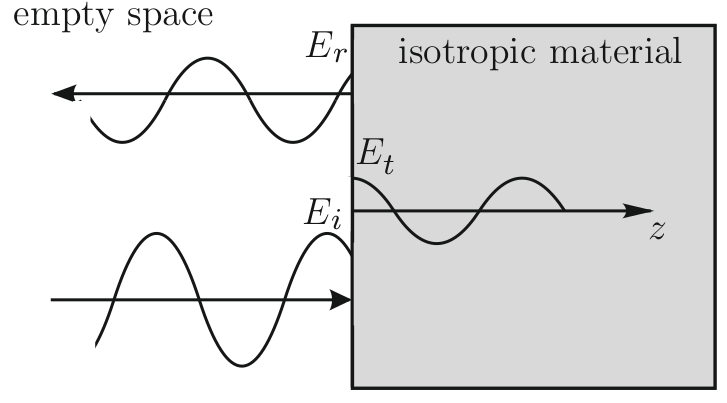
\includegraphics[height=1.2in,width=1.8in,viewport=0 0 750 600,clip]{Figures/Optic-reflect.png}
\caption{\small \textrm{Schematic representation of incident, reflected and transmitted electromagnetic wave at the surface.}}%
\label{Optic-reflect}
\end{figure} 
			\begin{displaymath}
				\begin{aligned}
					&E(z)=E_t\mathrm{e}^{\mathrm{i}(\omega/c)Nz}\quad z>0\\
					&E(z)=E_i\mathrm{e}^{\mathrm{i}(\omega/c)z}+E_r\mathrm{e}^{-\mathrm{i}(\omega/c)z}\quad z<0\\
				\end{aligned}
			\end{displaymath}
			反射率$R$可以表示为
			\begin{displaymath}
				R=\left|\frac{E_r}{E_i}\right|^2=\left|\frac{1-N}{1+N}\right|^2=\frac{(n-1)^2+k^2}{(n+1)^2+k^2}
			\end{displaymath}
	\end{itemize}
}

\subsection{自由载流子与\rm{Drude}模型}
\frame
{
	\frametitle{自由电子的\textrm{Drude}模型}
	\textcolor{blue}{在远红外区,经典自由电子气模型可以很好地描述金属的光学行为}
	\begin{itemize}
		\item 载流子在外电场$\mathbf{E}(\vec r,t)=\mathbf{E}_0\mathrm{e}^{\mathrm{i}(\vec q\cdot\vec r-\omega t)}$下的运动方程
			\begin{displaymath}
				m\ddot{\vec r}=-\frac m{\tau}\dot{\vec r}+(-e)\mathbf{E}_0\mathrm{e}^{\mathrm{i}(\vec q\cdot\vec r-\omega t)}
			\end{displaymath}
			这里$\vec r(t)$是载流子坐标,$\tau$是\textcolor{red}{唯象弛豫时间}
		\item 长波极限下,忽略电磁波在空间的变化
			\begin{displaymath}
				m\ddot{\vec r}=-\frac m{\tau}\dot{\vec r}-e\mathbf{E}_0\mathrm{e}^{\mathrm{i}-\omega t}
			\end{displaymath}
			取载流子位置函数$\vec r(t)=\vec A_0\mathrm{e}^{-\mathrm{i}\omega t}$,有
			\begin{displaymath}
				\vec A_0=\frac{e\tau}m\frac1{\omega(\mathrm{i}+\omega\tau)}\mathbf{E}_0
			\end{displaymath}
	\end{itemize}
}

\frame
{
	\frametitle{自由电子的\textrm{Drude}模型}
	如果载流子密度为$n$,则电流密度
	\begin{displaymath}
		\mathbf{J}=n(-e)\dot{\vec r}=n(-e)(-\mathrm{i}\omega)\vec A_0\mathrm{e}^{-\mathrm{i}\omega t}=\frac{ne^2\tau}m\frac1{1-\mathrm{i}\omega\tau}\mathbf{E}_0\mathrm{e}^{-\mathrm{i}\omega t}
	\end{displaymath}
	由此可得频率有关的电导率表示为
	\begin{displaymath}
		\sigma(\omega)=\frac{ne^2\tau}m\frac1{1-\mathrm{i}\omega\tau}=\sigma_0\frac1{1-\mathrm{i}\omega\tau}
	\end{displaymath}
	其中$\sigma_0=ne^2\tau/m$是静态电导率
	\begin{itemize}
		\item 介电函数可表示为
			\begin{displaymath}
				\varepsilon(\omega)=1-\frac{\omega_\mathrm{p}^2}{\omega(\omega+\mathrm{i}/\tau)}=\underline{\textcolor{blue}{\left[ 1-\frac{\omega_{\mathrm{p}}^2\tau^2}{1+\omega^2\tau^2} \right]}}+\mathrm{i}\underline{\textcolor{blue}{\left[ \frac{\omega_{\mathrm{p}}^2\tau}{\omega(1+\omega^2\tau^2)} \right]}}
			\end{displaymath}
			其中$\omega_{\mathrm{p}}$是载流子的等离振荡频率
			\begin{displaymath}
				\omega_{\mathrm{p}}^2=\frac{4\pi ne^2}m
			\end{displaymath}
%\begin{displaymath}
%	\epsilon_1(\omega)=1-\frac{\omega_{\mathrm{p}}^2\tau^2}{1+\omega^2\tau^2}\quad \epsilon_2(\omega)=\frac{\omega_{\mathrm{p}}^2\tau}{\omega(1+\omega^2\tau^2)}\quad
%\end{displaymath}
	\end{itemize}
}

\subsection{固体的光吸收过程}
\frame
{
\frametitle{带间跃迁的计算}
\begin{itemize}
\setlength{\itemsep}{10pt}
	\item 用半经典方法处理周期性体系的光学性质,用量子力学处理介质,对电磁波仍然采用经典电动力学描写
	\item 以半导体中的带间垂直跃迁(价带$|v,\vec k\rangle$,导带$|c,\vec k\rangle$)为例讨论固体的能带间跃迁
\begin{figure}[h!]
\centering
%\hspace*{-10pt}
\vspace*{-0.3in}
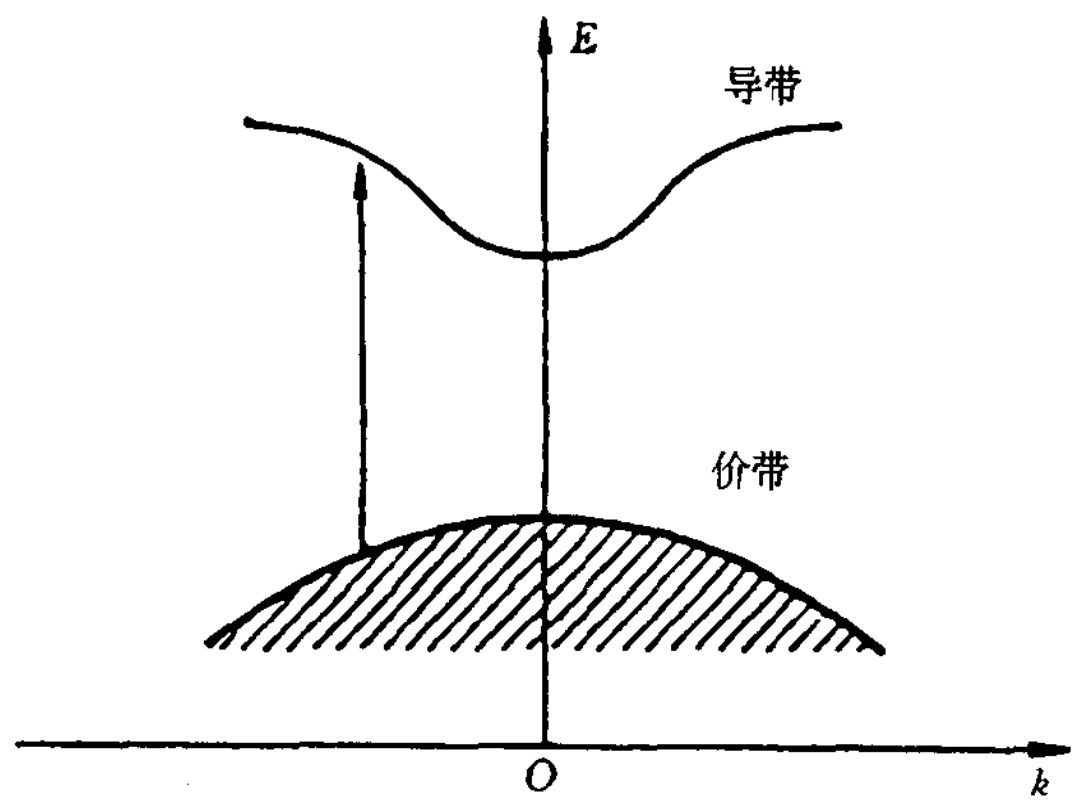
\includegraphics[height=1.8in,width=2.0in,viewport=0 0 1000 900,clip]{Figures/optic_dir.png}
\caption{\small \textrm{Schematic representation of directly inter-band transition.}}%
\label{Optic-dir}
\end{figure} 
\end{itemize}
}

\frame
{
	\frametitle{带间跃迁的计算}
\begin{itemize}
晶体中动量为$\vec p$的电子在电磁场(电磁场矢量势为$\vec A$)存在情况下,应用含时微扰理论,
\begin{displaymath}
	\hspace*{-20pt}
	H=\frac1{2m}[\vec p+\frac{e}c\mathbf{A}(\vec r,t)]^2+V(\vec r)=\left[ \frac{\vec p^2}{2m}+V(\vec r) \right]+\frac{e}{mc}\mathbf{A}\cdot\vec p+\frac{e^2}{2mc^2}\mathbf{A}^2
\end{displaymath}
其中电磁波
\begin{displaymath}
	\mathbf{A}(\vec r,t)=A_0\mathbf{e}\mathrm{e}^{\mathrm{i}(\vec q\cdot\vec r-\omega t)}+\mathrm{c.c}\quad\mathbf{e}\bot\vec q
\end{displaymath}
准确到$\vec A$的线性项(忽略$\vec A$的平方项)\textrm{Hamiltonian}为:
\begin{displaymath}
	H=\left[ \frac{\vec p^2}{2m}+V(\vec r) \right]+\frac{eA_0}{mc}\mathrm{e}^{\mathrm{i}(\vec q\cdot\vec r-\omega t)}\mathbf{e}\cdot\vec p+\frac{eA_0}{mc}\mathrm{e}^{-\mathrm{i}(\vec q\cdot\vec r-\omega t)}\mathbf{e}\cdot\vec p
\end{displaymath}
	\item 频率为$\omega$的平面偏振光,电场和磁场的强度为
\begin{displaymath}
%  \left\{
\begin{aligned}
    \vec E&=-\frac1c\frac{\partial\vec A}{\partial t}\\
    \vec B&=\nabla\times\vec A
  \end{aligned}%\right.
  \label{eq:optic-26}
\end{displaymath}
\end{itemize}
%式中$c$为光速。
}

\frame
{
\frametitle{带间跃迁的计算}
在含时微扰\textrm{Hamiltonian}作用下,带间垂直跃迁为
\begin{displaymath}
	\begin{aligned}
		W(\vec q,\omega)=&\frac{2\pi}{\hbar}\left( \frac{eA_0}{m_ec} \right)^22\sum_{i,j}|\langle c,\vec k|\mathrm{e}^{\mathrm{i}\vec q\cdot\vec r}\mathbf{e}\cdot\vec p|v,\vec k\rangle|^2\\
		\times&\delta[E_c(\vec k)-E_v(\vec k)-\omega][f(E_c(\vec k))-f(E_v(\vec k))]
	\end{aligned}
  \label{eq:optic-27}
\end{displaymath}
$\delta$因子表示跃迁过程的能量守恒关系%,矩阵元$\langle c\vec k|H'|v\vec k\rangle$表示\textrm{Bloch}函数间的积分
。对垂直跃迁,忽略磁场贡献,%矩阵元可以简写成$\dfrac1cA_0\vec e\cdot\vec M_{cv}(\vec k)$,$\vec s$为电磁波矢量势$\vec A_0(=A_0\vec s)$方向的单位矢量。
只有满足能量守恒和动量守恒条件的跃迁才对积分有贡献。%$\displaystyle\int W\dfrac{\textrm{d}\vec k}{(2\pi)^3}$为单位体积、单位时间内吸收能量为$\omega$的光子的总数,系数2是考虑两种自旋态。将式\eqref{eq:optic-27},\eqref{eq:optic-28}代入式\eqref{eq:optic-29},并应用$\dfrac{A_0}c\vec e\cdot\vec M_{cv}(\vec k)$表示矩阵元,得

电磁波在介质中产生的电场
\begin{displaymath}
	\mathbf{E}(\vec r,t)=-\frac1c\frac{\partial\mathbf{A}}{\partial t}=E_0\mathbf{e}\mathrm{e}^{\mathrm{i}\vec q\cdot\vec r-\omega t}+\mathrm{c.c}\quad\mbox{其中}E_0=\mathrm{i}\omega\frac{A_0}c
\end{displaymath}

介质中的传导电流
\begin{displaymath}
	\mathbf{J}(\vec r,t)=\sigma(\vec q,\omega)E_0\mathbf{e}\mathrm{e}^{\mathrm{i}(\vec q\cdot\vec r-\omega t)}+\mathrm{c.c}\quad(\mathbf{e}\bot\vec q)
\end{displaymath}
由此计算得到吸收功率
\begin{displaymath}
	\int_V\mathbf{J}\cdot\mathbf{E}\mathrm{d}\vec r=2\sigma_1(\vec q,\omega)|E_0|^2V=2\sigma_1(\vec q,\omega)\frac1{c^2}\omega^2A_0^2V=\textcolor{blue}{\hbar\omega W(\vec q,\omega)}
\end{displaymath}
}

\frame
{
	\frametitle{带间跃迁的计算}
长波极限下($\vec q\rightarrow0$), 根据光学性质的基本关系,可有介电函数的介电函数虚部表达式
\begin{displaymath}
	\begin{aligned}
		\varepsilon_2(\omega)=&\lim_{\vec q\rightarrow0}\frac{8\pi^2e^2}{m_e^2\omega^2}\int\frac{\mathrm{d}\vec k}{(2\pi)^3}|\langle c,\vec k|\mathbf{e}\cdot\vec p|v,\vec k\rangle|^2\\
		\times&\delta(E_c(\vec k)-E_v(\vec k)-\hbar\omega)[f(E_c(\vec k))-f(E_v(\vec k))]
	\end{aligned}
  \label{eq:optic-varepsilon_2}
\end{displaymath}
$\varepsilon_2(\omega)$是晶体的光学吸收和能带结构之间的基本关系

对应的$\varepsilon_1$可以根据\textrm{Kramers-Kr\"onig}关系%\eqref{eq:optic-16}
得到
\begin{displaymath}
	\varepsilon_1(\omega)=1+\frac1{\pi}\mathscr{P}\int_{-\infty}^{+\infty}\frac{\varepsilon_2(\omega^{\prime})}{\omega^{\prime}-\omega}\textrm{d}\omega^{\prime}=1+\frac2{\pi}\mathscr{P}\int_0^{+\infty}\frac{\omega^{\prime}\varepsilon_2(\omega^{\prime})}{\omega^{\prime2}-\omega^2}\textrm{d}\omega^{\prime}
  \label{eq:optic-varepsilon_1}
\end{displaymath}
因此介电函数表示为
\begin{displaymath}
	\hspace*{-10pt}
	\varepsilon(\omega)=1+\frac{8\pi e^2}{m_e^2}\int\frac{\mathrm{d}\vec k}{(2\pi)^3}\frac{|\langle c,\vec k|\mathbf{e}\cdot\vec p|v,\vec k\rangle|^2}{(E_c(\vec k)-E_v(\vec k))/\hbar^2}\frac{(-\mathrm{i})[f(E_c(\vec k))-f(E_v(\vec k))]}{E_c(\vec k)-E_v(\vec k)-\hbar\omega-\mathrm{i}\eta}
  \label{eq:optic-varepsilon}
\end{displaymath}
}

\frame
{
	\frametitle{带间跃迁和带内跃迁的计算}
电导率函数可表示为
\begin{displaymath}
	\sigma(\omega)=\frac{2e^2}{m_e^2}\int\frac{\mathrm{d}\vec k}{(2\pi)^3}\frac{|\langle c,\vec k|\mathbf{e}\cdot\vec p|v,\vec k\rangle|^2}{(E_c(\vec k)-E_v(\vec k))/\hbar}\frac{(-\mathrm{i})[f(E_c(\vec k))-f(E_v(\vec k))]}{E_c(\vec k)-E_v(\vec k)-\hbar\omega-\mathrm{i}\eta}
  \label{eq:optic-sigma}
\end{displaymath}

\textcolor{violet}{推广到长波极限下的带内跃迁}
\begin{displaymath}
	f(E_c(\vec k))-f(E_v(\vec k))\approx\frac{\partial f}{\partial E}(f(E_c(\vec k))-f(E_v(\vec k)))
\end{displaymath}
\begin{displaymath}
	\sigma(\omega)=\frac{e^2\hbar}{4\pi^3}\int\mathrm{d}\vec k\langle c,\vec k|\mathbf{e}\cdot\vec p|v,\vec k\rangle|^2\frac{-\mathrm{i}}{E_c(\vec k)-E_v(\vec k)-\hbar\omega-\mathrm{i}\eta}\left( -\frac{\partial f}{\partial E} \right)
\end{displaymath}
引入等式$\eta=\hbar/\tau$,并作展开
\begin{displaymath}
	E_{\vec k+\vec q}-E_{\vec k}\approx\vec q\cdot(\partial E/\partial\vec k)=\frac{\hbar}{m_e}\langle c,\vec k|\mathbf{q}\cdot\vec p|v,\vec k\rangle
\end{displaymath}
由此可得
\vspace{-5pt}
\begin{displaymath}
	\sigma(\vec q,\omega)=\frac{e^2}{4\pi^3}\int\mathrm{d}\vec k\frac{\tau|\langle c,\vec k|\mathbf{e}\cdot\vec p|v,\vec k\rangle|^2}{1-\mathrm{i}\tau(\omega-\langle c,\vec k|\mathbf{q}\cdot\vec p|v,\vec k\rangle)}\left( -\frac{\partial f}{\partial E} \right)
\end{displaymath}
}

\frame
{
\frametitle{联合态密度(Joint DOS, JDOS)}
定义联合态密度(\textrm{Joint Density of States, JDOS})
\begin{displaymath}
  J_{cv}(\hbar\omega)=\sum_{v,c}\int\delta[E_c(\vec k)-E_v(\vec k)-\omega]\frac{2\textrm{d}\vec k}{(2\pi)^3}
  \label{eq:optic-33}
\end{displaymath}
令$E_{cv}(\vec k)$\,=\,$E_c(\vec k)-E_v(\vec k)$,因$\textrm{d}\vec k$\,=\,$\dfrac{dE_{cv}(\vec k)}{\nabla_{\vec k}E_{cv}(\vec k)}\textrm{d}S$,故有
\begin{displaymath}
  J_{cv}(\omega)=\frac2{(2\pi)^3}\sum_{v,c}\int\limits_{E_{cv}(\vec k)=\omega}\frac{\textrm{d}S}{\nabla_{\vec k}E_{cv}(\vec k)}
  \label{eq:optic-34}
\end{displaymath}
类似态密度的定义,而$E_{cv}(\vec k)$同时联系着价带和导带,因此称为联合态密度。当矩阵元$\vec M_{cv}(\vec k)$随波矢$\vec k$变化比较小的时候,可以近似地认为$\varepsilon_2(\omega)\!\propto\!J_{cv}(\omega)$。满足$|\nabla_{\vec k}E_{cv}(\vec k)|\!=\!0$的$\vec k$点,是联合态密度$J_{cv}(\omega)$和$\varepsilon_2(\omega)$的奇点(\textrm{Van Hove}奇点或临界点),在这些点,$J_{cv}(\omega)$和$\varepsilon_2(\omega)$%的能谱图将出现典型结构(即
对能量的微商呈现典型的不连续。%联合态密度的奇点有两种情况,即$\nabla_{\vec k}E_c(\vec k)\!=\!\nabla_{\vec k}E_v(\vec k)\!=\!0$和$\nabla_{\vec k}E_c(\vec k)\!=\!\nabla_{\vec k}E_v(\vec k)\!\neq\!0$。将$E_{cv}(\vec k)$在奇点作Taylor级数展开到二级,$$E_{cv}(\vec k)=E_0+a_xk_x^2+a_yk_y^2+a_zk_z^2$$可以看出有四种类型的奇点:
}

\section{\rm{Wannier function}}
\frame
{
	\frametitle{\textrm{Wannier~}函数}
	\begin{itemize}
		\item \textrm{Wannier}函数是\textcolor{blue}{正交化的局域函数},\textcolor{red}{要求局域函数空间与能带空间完全相同}
		\item 紧束缚近似下,能带的电子波函数的\underline{\textcolor{blue}{\textrm{Bloch~}和}}
			\begin{displaymath}
				\psi_i^{\vec k}(\vec r)=\frac1{\sqrt N}\sum_m\mathrm{e}^{\mathrm{i}\vec k\cdot\vec R_m}\phi_i(\vec r-\vec R_m)
			\end{displaymath}
		\textrm{Bloch~}函数可以写类似形式
		\begin{displaymath}
			\psi_i^{\vec k}(\vec r)=\frac1{\sqrt N}\sum_m\mathrm{e}^{\mathrm{i}\vec k\cdot\vec R_m}W_i(\vec r-\vec R_m) 
		\end{displaymath}
		这里$W_i(\vec r-\vec R_n)$就是\textrm{Wannier~}函数
	\end{itemize}
}

\frame
{
	\frametitle{\textrm{Wannier~}函数}
	\begin{itemize}
		\item \textrm{Wannier~}函数是\textrm{Bloch~}函数的\textrm{Fourier}变换,对于格点$\vec T_m$有
			\begin{displaymath}
				\begin{aligned}
					&w_i(\vec r-\vec T_m)=\frac{\Omega_{\mathrm{cell}}}{2\pi^3}\int_{\mathrm{BZ}}\mathrm{d}\vec k\mathrm{e}^{-\mathrm{i}\vec k\cdot\vec T_m}\psi_i^{\vec k}(\vec r)\\
					=&\frac{\Omega_{\mathrm{cell}}}{2\pi^3}\int_{\mathrm{BZ}}\mathrm{d}\vec k\mathrm{e}^{-\mathrm{i}\vec k\cdot\vec T_m}\mathrm{e}^{-\mathrm{i}\vec k\cdot\vec r}u_i^{\vec k}(\vec r)=\frac{\Omega_{\mathrm{cell}}}{2\pi^3}\int_{\mathrm{BZ}}\mathrm{d}\vec k\mathrm{e}^{\mathrm{i}\vec k\cdot(\vec r-\vec T_m)}u_i^{\vec k}(\vec r)
				\end{aligned}
			\end{displaymath}
\begin{figure}[h!]
\centering
%\hspace*{-10pt}
\vspace*{-0.6in}
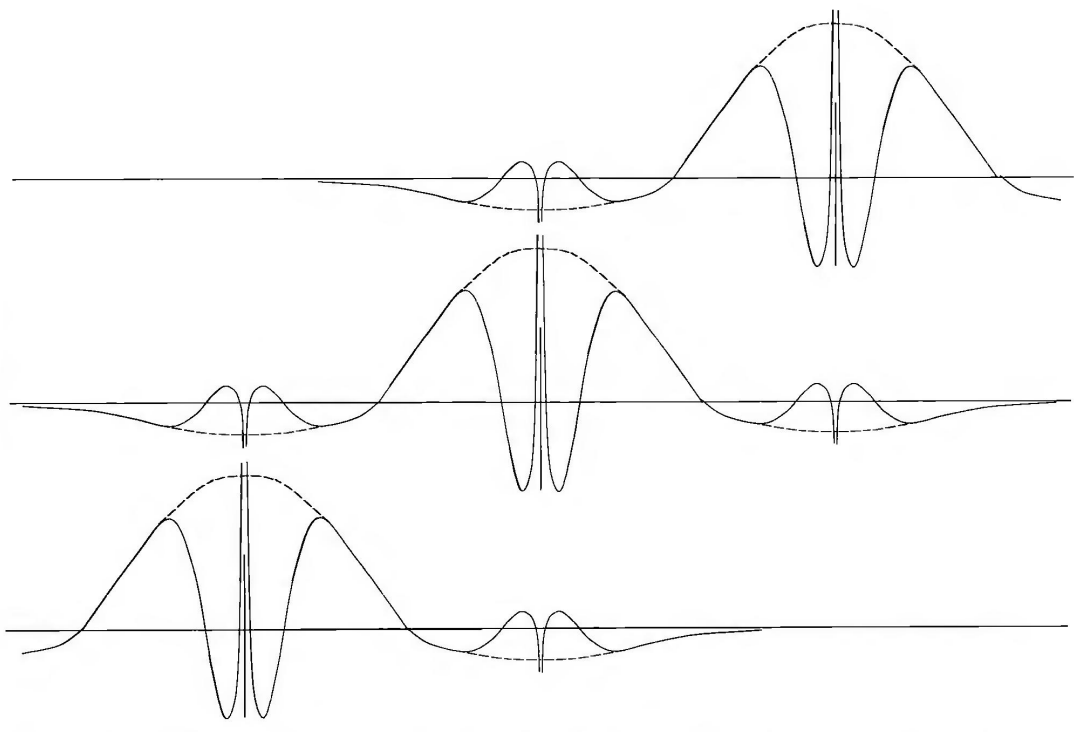
\includegraphics[height=1.8in,width=3.1in,viewport=0 0 1400 1000,clip]{Figures/Wannier_function.png}
\caption{\small \textrm{Schematic example of Wannier function that correspond to the Bloch function.}}%
\label{Wannier-function}
\end{figure} 
	\end{itemize}
}

\frame
{
	\frametitle{\textrm{Wannier~}函数}
	\begin{itemize}
		\item 一个能带的\textrm{Wannier~}函数完全由同一能带的\textrm{Bloch~}函数定义
		\item \textrm{Wannier~}函数完全正交
			\begin{displaymath}
				\int_{\textcolor{red}{\mathrm{all\; space}}}\mathrm{d}\vec rw_i^{\ast}(\vec r-\vec T_m)w_j(\vec r-\vec T_{m^{\prime}})=\delta_{ij}\delta_{mm^{\prime}}
			\end{displaymath}
			\textrm{Wannier~}函数和\textrm{Bloch~}函数一样,构成完备的正交函数集
		\item \textrm{Wannier~}函数间由幺正矩阵联系
			\begin{displaymath}
				u_{i\vec k}=\sum_jU_{ji}^{\vec k}u_{j\vec k}^{(0)}
			\end{displaymath}
			\textcolor{blue}{其中$U_{ji}^{\vec k}$是与$\vec k$~关联的幺正矩阵}
	\end{itemize}
}

\frame
{
	\frametitle{\textrm{Wannier~}函数的不唯一}
	\begin{itemize}
		\item 对于\textrm{Bloch~}函数
			\begin{displaymath}
				\psi_i^{\vec k}(\vec r)=\mathrm{e}^{\mathrm{i}\vec k\cdot\vec r}\mathrm{e}^{-\mathrm{i}\vec k\cdot\vec r}u_i^{\vec k}(\vec r)
			\end{displaymath}
			\textcolor{red}{可乘以任意相位,而不改变物理量的值}
			\begin{displaymath}
				\psi_i^{\vec k}(\vec r)\rightarrow\tilde\psi_i^{\vec k}(\vec r)=\textcolor{red}{\mathrm{e}^{\mathrm{i}\phi_i(\vec k)}}\psi_i^{\vec k}(\vec r)
			\end{displaymath}
		\item \textcolor{blue}{\textrm{Wannier~}函数的表示并不唯一}:\\
必须通过选择特定的相位$\phi_i(\vec k)$(或特定的幺正变换矩阵),才能得到确定的\textrm{Wannier~}函数 
\begin{figure}[h!]
\centering
%\hspace*{-10pt}
\vspace*{-0.3in}
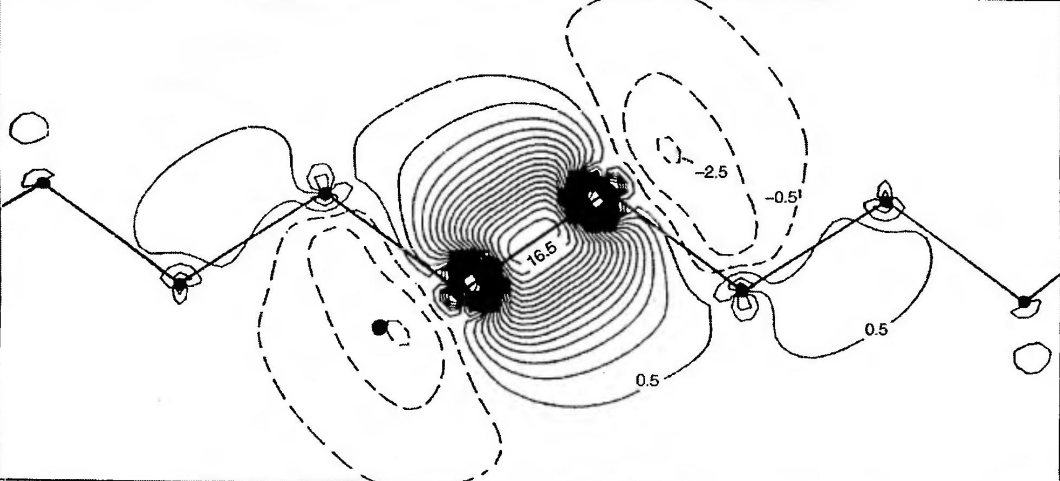
\includegraphics[height=1.1in,width=1.8in,viewport=0 0 1100 600,clip]{Figures/Wannier_function-Bondcenter_Si.png}
\caption{\small \textrm{Bond-centered Wannier function for Si.}}%
\label{Bond-Centered Wannier function}
\end{figure} 
	\end{itemize}
}

\frame
{
	\frametitle{\textrm{Wannier~}函数的不唯一}
\begin{figure}[h!]
\centering
\hspace*{-0.35in}
\subfigure[\textrm{Maximally localized Wannier function}]{
\label{Brillouin_Zone_Cubic}
\vspace*{-0.50in}
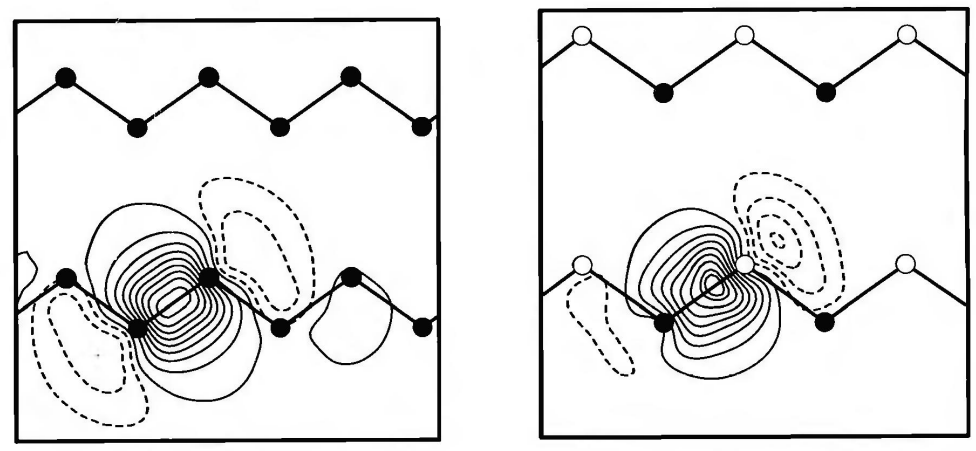
\includegraphics[height=1.10in,width=3.20in,viewport=0 0 1000 450,clip]{Figures/Wannier_function-Maxlocal.png}}
\subfigure[\textrm{Comparison of orthogonal and non-orthogonal maximally locaized orbitals}]{
\label{Band_Gap_SrSnO3}
\vspace*{-0.50in}
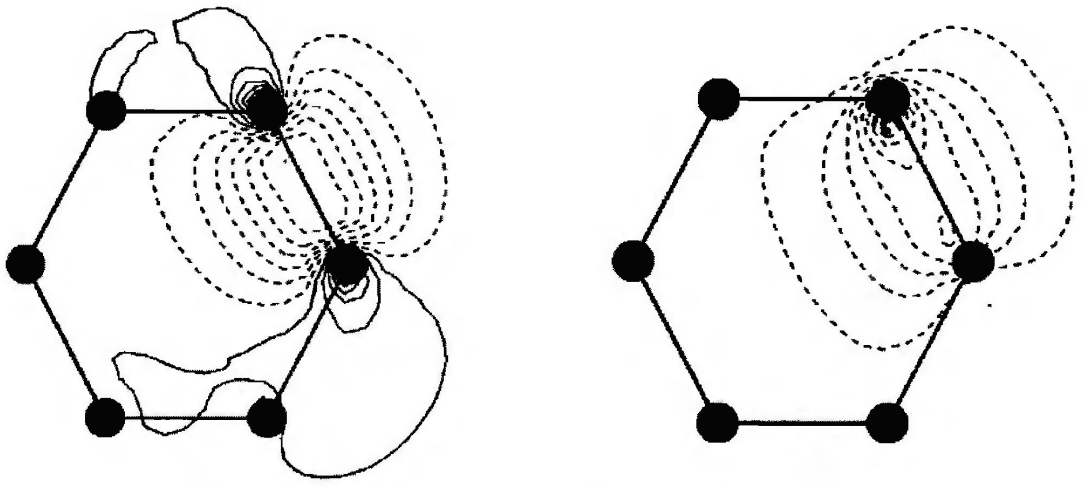
\includegraphics[height=1.10in,width=3.00in,viewport=0 0 1200 550,clip]{Figures/Non_orth-Wannier_function.png}}
\label{Non-local Wannier-function}
\end{figure}
}

\section{极化与\rm{Berry~}相位}
\frame
{
	\frametitle{电介质材料的极化}
	\textcolor{blue}{电极化}:~电介质内部正负电荷的相对位移,会产生电偶极子,这现象称为电极化
	\begin{itemize}
\setlength{\itemsep}{10pt}
		\item \textcolor{red}{压电效应}:~\textcolor{blue}{电介质沿一定方向受外力发生形变时,内部会产生极化现象:~在电解质两个相对表面出现正负相反电荷;当作用力方向改变时,电荷的极性也随之改变;当外力去掉后,又会恢复到不带电的状态}
		\item \textcolor{red}{热电效应}:~\textcolor{blue}{电介质因为受热,电子(空穴)由高温区往低温区移动时,产生电荷堆积引起极化}
		\item \textcolor{red}{铁电效应}:~\textcolor{blue}{某些电介质中,晶胞的结构使正负电荷中心不重合而出现电偶极矩,在内部产生非零的电极化强度,使晶体具有自发极化,且电偶极矩方向可以因外电场而改变,呈现出类似于铁磁体的特点}
	\end{itemize}
}

\frame
{
	\frametitle{外电场下的极化}
	\begin{itemize}
		\item 金属在外电场下的极化
\begin{figure}[h!]
\centering
%\hspace*{-10pt}
\vspace*{-0.15in}
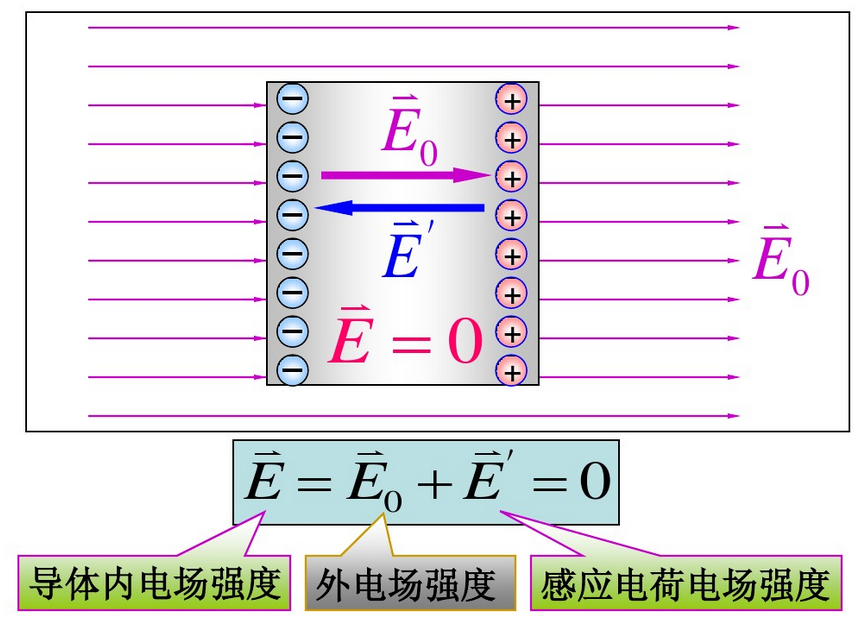
\includegraphics[height=1.8in,width=3.3in,viewport=0 0 1100 650,clip]{Figures/Polarize_metal-2.png}
\caption{\small \textrm{Schematic of a metal in the static electric field.}}%
\label{Polarization_metal}
\end{figure} 
\textcolor{blue}{金属体相的物理性质不会受外场的影响}
	\end{itemize}
}

\frame
{
	\frametitle{外电场下的极化}
	\begin{itemize}
		\item 绝缘体在外电场下的极化\\
			根据电磁理论,电场极化强度可定义为
			\begin{displaymath}
				\nabla\cdot\vec P(\vec r,t)=-\delta n(\vec r,t)
			\end{displaymath}
			利用极化电流守恒条件$\nabla\cdot\mathbf{j}(\vec r,t)=-\mathrm{d}n(\vec r,t)/\mathrm{d}t$\\
			可得电场极化强度与极化电流密度关系
			\begin{displaymath}
				\frac{\mathrm{d}\vec P(\vec r,t)}{\mathrm{d}t}=\mathbf{j}(\vec r,t)+\nabla\times\mathbf{M}(\vec r,t)
			\end{displaymath}
			这里$\mathbf{M}(\vec r,t)$是任意矢量场

			宏观电场极化强度一般定义为:\\\textcolor{blue}{单位体积中分子电偶极矩的矢量和}
	\end{itemize}
	\textcolor{red}{这样定义的极化强度存在一定的问题}
}

\frame
{
	\frametitle{外电场下的极化}
			\begin{enumerate}
				\item 对于有限体系,上述定义的电场极化强度是合理的
\begin{figure}[h!]
\centering
%\hspace*{-10pt}
\vspace*{-0.15in}
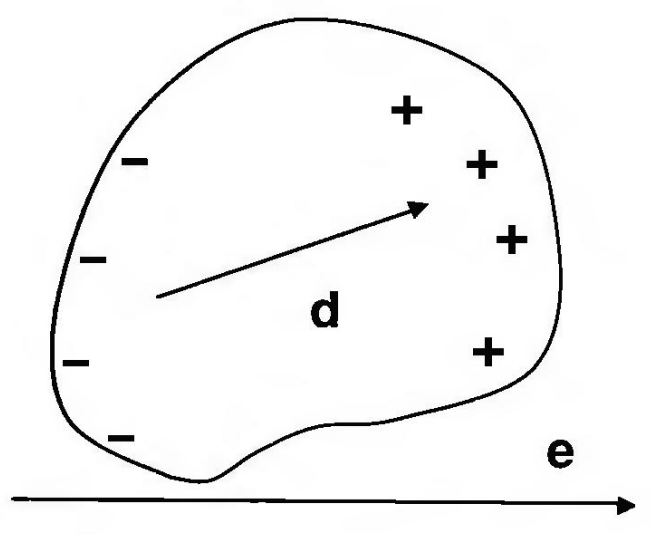
\includegraphics[height=0.9in,width=2.2in,viewport=0 0 1100 550,clip]{Figures/Polarize_insulator.png}
\caption{\small \textrm{Illustration of finite system for which the total dipole moment is well defined.}}%
\label{Polarization_insulator}
\end{figure} 
考虑到有限体系外$\vec P(\vec r)=0$,宏观电场极化强度$\vec P$可用偶极矩$\vec d$表示
\begin{displaymath}
	\vec P\equiv\frac{\vec d}{\Omega}=\frac1{\Omega}\int_{\mathrm{all\;space}}\mathrm{d}\vec rn(\vec r)\vec r
\end{displaymath}
\textcolor{red}{电场极化强度的变化$\Delta\vec P=\vec P^{(1)}-\vec P^{(0)}$只与电荷密度的改变$\Delta n=n^{(1)}-n^{(0)}$有关,而与电荷密度改变的路径有关}
			\end{enumerate}
}

\frame
{
	\frametitle{}
			\begin{enumerate}
				\setcounter{enumi}{1}
				\item 对于周期体系
\begin{figure}[h!]
\centering
%\hspace*{-10pt}
\vspace*{-0.15in}
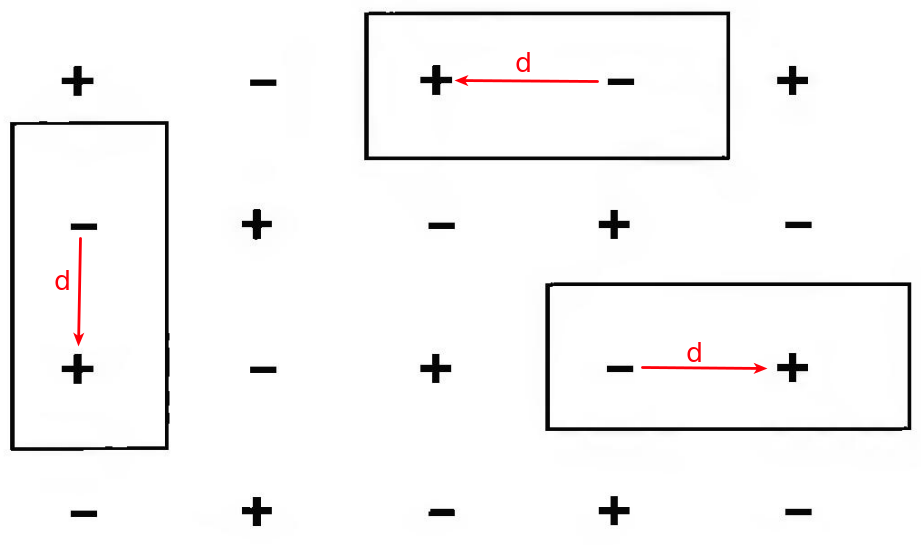
\includegraphics[height=0.9in,width=1.6in,viewport=0 0 1100 540,clip]{Figures/Polarize_insulator-2.png}
\caption{\small \textrm{Point charge model of an ionic crystal. The dipole is obviously not unique since the cells shown all have different moments.}}%
\label{Polarization_insulator-2}
\end{figure} 
正确定义周期体系的宏观电场极化强度,、\textcolor{red}{必须用合适的形式代替对$\vec r$的无限积分}\\
宏观极化电流是极化过程中唯一可观测的物理量,极化强度的变化$\vec P$可由体相极化电流计算
\begin{displaymath}
	\vec P(\vec r,t)=\int^t\mathrm{d}t^{\prime}\mathbf{j}_{\mathrm{int}}(\vec r,t^{\prime})
\end{displaymath}
			\end{enumerate}
}

\frame
{
	\frametitle{现代极化理论与几何\textrm{Berry~}相位}
	\begin{itemize}
		\item 用极化电流计算电场极化定义虽然正确,但不能证明电场极化强度与积分路径无关
		\item \textrm{King-Smith}和\textrm{Vanderbilt}提出了新的计算方案\upcite{PRB47-1651_1993}:\\
		\textcolor{red}{基本假设}:~连续的绝热变化可关联\textrm{Kohn-Sham}方程的\textrm{Hamiltonian}描述的不同态\\如果满足条件
	\begin{enumerate}
		\item 没有任何外部电场存在 
		\item 体系始终保持绝缘体状态
	\end{enumerate}
	宏观电场极化极化强度的变化可表示为
	\begin{displaymath}
		\Delta\vec P=\int_0^1\mathrm{d}\lambda\frac{\partial\vec P}{\partial\lambda}
	\end{displaymath}
	\textcolor{red}{注意}:~对所有的$\lambda$,宏观外电场要求为0
	\end{itemize}
}

\frame
{
	\frametitle{现代极化理论与几何\textrm{Berry~}相位}
	\begin{itemize}
		\item 根据线性响应理论,\textrm{Resta}指出:~在无限体系中,微扰项$\partial\vec P/\partial\lambda$可以用动量矩阵元表示\upcite{RMP66-899_1994}
	\begin{displaymath}
		\frac{\partial\vec P}{\partial\lambda}=-\mathrm{i}\frac{\mathrm{e}\hbar}{\Omega m_e}\sum_{\vec k}\sum_i^{\mathrm{occ}}\sum_j^{\mathrm{empty}}\frac{\langle\psi_{\vec k i}^{\lambda}|\hat{\vec p}|\psi_{\vec k j}^{\lambda}\rangle\langle\psi_{\vec k i}^{\lambda}|\partial V_{\mathrm{KS}}^{\lambda}/\partial\lambda|\psi_{\vec k j}^{\lambda}\rangle}{(\varepsilon_{\vec k i}^{\lambda}-\varepsilon_{\vec k j}^{\lambda})^2}+\mathrm{c.c.}
	\end{displaymath}
	这里对$i,j$的求和遍历所有自旋态
	\item 早先\textrm{Thouless}等在讨论量子\textrm{Hall~}效应时曾证明,上述对所有态的求和可变换成只对占据态的求和\upcite{PRL49-405_1982}\\引入与$\vec k$有关的\textrm{Kohn-Sham~}势$V_{\mathrm{KS}}^{(\lambda)}(\vec r)$,因此周期性\textrm{Hamiltonian~}表示为
	\begin{displaymath}
		\hat H(\vec k,\lambda)=\frac1{2m_e}\left( -\mathrm{i}\hbar\nabla+\hbar\vec k \right)^2+V_{\mathrm{KS}}^{(\lambda)}(\vec r)
	\end{displaymath}
	\end{itemize}
}

\frame
{
	\frametitle{现代极化理论与几何\textrm{Berry~}相位}
	利用\textrm{Bloch~}函数
	\begin{displaymath}
		\psi_{\vec k i}^{\lambda}=\mathrm{e}^{\mathrm{i}\vec k\cdot\vec r}u_{\vec k i}^{\lambda}(\vec r)
	\end{displaymath}
	满足等式
	\begin{displaymath}
		\hat H(\vec k,\lambda)u_{\vec k i}^{\lambda}(\vec r)=\left[ -\frac{\hbar}{2m_e}(\nabla+\mathrm{i}\vec k)^2 +V_{\mathrm{KS}}^{(\lambda)}(\vec r)\right]u_{\vec k i}^{\lambda}(\vec r)=\varepsilon_{\vec k i}^{\lambda}u_{\vec k i}^{\lambda}(\vec r)
	\end{displaymath}
	根据\textcolor{red}{对易关系}
	\begin{displaymath}
		\langle\psi_{\vec k i}^{\lambda}|\hat{\vec p}|\psi_{\vec k j}^{\lambda}\rangle=\frac{m_e}{\hbar}\langle u_{\vec k i}^{\lambda}|[\partial/\partial\vec k,\hat H(\vec k,\lambda)]|u_{\vec k j}^{\lambda}\rangle
	\end{displaymath}
	\begin{displaymath}
		\langle\psi_{\vec k i}^{\lambda}|\partial V_{\mathrm{KS}}^{\lambda}/\partial\lambda|\psi_{\vec k j}^{\lambda}\rangle=\frac{m_e}{\hbar}\langle u_{\vec k i}^{\lambda}|[\partial/\partial\lambda,\hat H(\vec k,\lambda)]|u_{\vec k j}^{\lambda}\rangle
	\end{displaymath}
	可得
	\begin{displaymath}
		\Delta\vec P_{\alpha}=-|e|\frac2{(2\pi)^3}\mathrm{Im}\int_{\mathrm{BZ}}\mathrm{d}\vec k\int_0^1\mathrm{d}\lambda\sum_i^{\mathrm{occ}}\left\langle\frac{\partial u_{\vec k i}^{(\lambda)}}{\partial k_{\alpha}}\right|\left.\frac{\partial u_{\vec k j}^{(\lambda)}}{\partial\lambda}\right\rangle
	\end{displaymath}
	对$\vec k$~的积分是倒空间的第一\textrm{Brillouin zone}
}

\frame
{
	\frametitle{现代极化理论和几何\textrm{Berry~}相位}
	\textrm{Thouless~}在讨论无相互作用粒子的量子\textrm{Hall~}效应时曾给出类似的积分表达式\upcite{PRB27-6083_1983},利用\textrm{Stokes~}定律
\begin{figure}[h!]
\centering
%\hspace*{-10pt}
\vspace*{-0.12in}
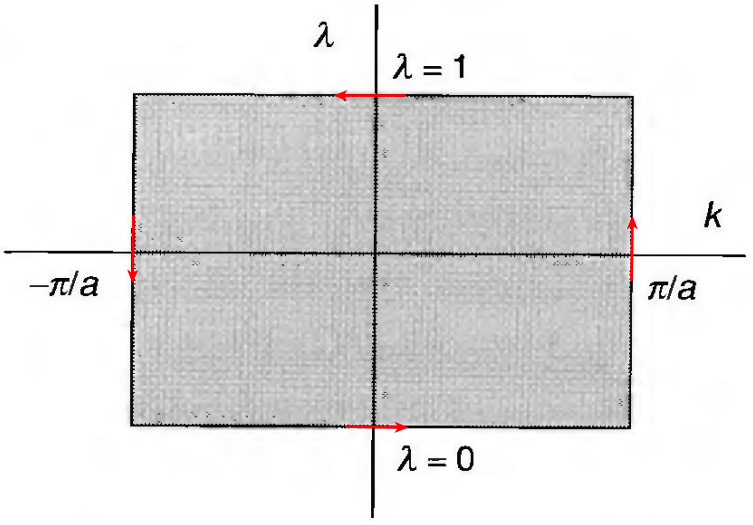
\includegraphics[height=1.2in,width=1.6in,viewport=0 0 800 540,clip]{Figures/Berry_contour_integration.png}
\caption{\small \textrm{Schematic figure of region of integration in $(k,\lambda)$ space for calculation of $\Delta P$ using the contour of integration C.}}%
\label{Berry_contour_integration}
\end{figure} 
	\begin{displaymath}
		\Delta P=-|e|\frac2{(2\pi)^3}\mathrm{Im}\sum_i^{\mathrm{occ}}\left\{ \underline{\textcolor{blue}{\oint_C\sum_{j=1}^2\mathrm{d}\tau_j\langle u_{k i}^{\lambda}|\partial/\partial\tau_j|u_{k i}^{\lambda}\rangle}} \right\} 
	\end{displaymath}
这里$\tau$~是二维空间$(\lambda,k)$,$C$是$\tau$空间的围道
}

\frame
{
	\frametitle{现代极化理论和几何\textrm{Berry~}相位}
	\begin{itemize}
		\item 上述大括号内的积分是\textcolor{red}{绝热近似下,利用周期波函数围道积分计算的\textrm{Berry~}相位改变}\upcite{PRS392-45_1984,PRL51-2167_1983}
		\item \textrm{Thouless~}指出上述围道积分对应的是在势$V_{\mathrm{KS}}^{(0)}=V_{\mathrm{KS}}^{(1)}$条件下的积分,\textcolor{blue}{围道积分计算的是实空间波函数点的相位变化}
		\item 考虑到波函数的周期性,用$(k,\lambda)$表示的相位变化可以加$2n\pi$而不变
	\end{itemize}
	利用周期函数$u_{\vec k i}^{(\lambda)}$的“周期标度关系”
	\begin{displaymath}
		u_{\vec k+\vec G i}^{(\lambda)}(\vec r)=\textcolor{green}{\mathrm{e}^{\mathrm{i}\vec G\cdot\vec r}}u_{\vec k i}^{(\lambda)}(\vec r)
	\end{displaymath}
	其中$\vec G$是倒空间格矢,因此这种标度关系并不唯一
%	选择$\vec G$满足在$\vec k$和$\vec k+\vec G$对$\lambda$的二重积分相互抵消,因此
	\begin{displaymath}
		\Delta\vec P_{\alpha}=\mathrm{i}\frac{-|e|}{(2\pi)^3}\sum_i^{\mathrm{occ}}\int_{\mathrm{BZ}}\mathrm{d}\vec k\left[ \langle u_{\vec k i}^{\lambda=1}|\partial/\partial_{k_{\alpha}}|u_{\vec k i}^{\lambda=1}\rangle-\langle u_{\vec k i}^{\lambda=0}|\partial/\partial_{k_{\alpha}}|u_{\vec k i}^{\lambda=0}\rangle \right]
	\end{displaymath}
}

\frame
{
	\frametitle{现代极化理论和几何\textrm{Berry~}相位}
	利用周期标度关系,可有
	\begin{displaymath}
		\Delta\vec P=\vec P^{(1)}-\vec P^{(0)}	
	\end{displaymath}
	其中
	\begin{displaymath}
		P_{\alpha}^{(\lambda)}=\mathrm{i}\frac{-|e|}{(2\pi)^3}\sum_i^{\mathrm{occ}}\int_{\mathrm{BZ}}\mathrm{d}\vec k\langle u_{\vec k i}^{(\lambda)}|\partial/\partial_{k_{\alpha}}|u_{\vec k i}^{(\lambda)}\rangle
	\end{displaymath}
	\textrm{Zak~}等指出,\textcolor{red}{上述表达式即能带$i$的\textrm{Berry~}相位}\upcite{PRL62-2747_1989,EPL18-239_1992}
	
	\textcolor{blue}{注意到\textrm{Wannier~}函数的形式与“周期标度”的相位密切相关},有
	\begin{displaymath}
		u_{\vec k i}^{(\lambda)}(\vec r)=\frac 1{\sqrt N}\sum_{\vec R}\mathrm{e}^{-\mathrm{i}\vec k\cdot(\vec r-\vec R)}w_i^{(\lambda)}(\vec r-\vec R)
	\end{displaymath}
	利用\textrm{Wannier~}函数,$P_{\alpha}^{(\lambda)}$可以具有更简单的形式
	\begin{displaymath}
		\vec P^{(\lambda)}=-\frac{2e}{\Omega}\sum_i^{\mathrm{occ}}\int\vec r|w_i^{(\lambda)}(\vec r)|^2\mathrm{d}\vec r
	\end{displaymath}
	这里$\Omega$是原胞体积
}

\frame
{
	\frametitle{现代极化理论和几何\textrm{Berry~}相位}
	\textcolor{red}{电介质的极化改变正比于由绝热变化引起的\textrm{Wannier~}函数的电荷中心的偏移}

	考虑到绝热变化要求$V_{\mathrm{KS}}^{(0)}=V_{\mathrm{KS}}^{(1)}$,因此周期函数$u_{\vec k i}^{(0)}$和$u_{\vec k i}^{(1)}$仅有相位的差别
	\begin{displaymath}
		u_{\vec k i}^{(1)}=\mathrm{e}^{\mathrm{i}\theta_{\vec k i}}u_{\vec k i}^{(\lambda)}
	\end{displaymath}
	因此
	\begin{displaymath}
		\Delta P_{\alpha}=-\frac{|e|}{(2\pi)^3}\sum_i^{\mathrm{occ}}\int_{\mathrm{BZ}}\mathrm{d}\vec k\partial\theta_{\vec k i}/\partial k_{\alpha}
	\end{displaymath}
	$\mathrm{e}^{\mathrm{i}\theta_{\vec k i}}$是$\vec k$的周期函数,最一般的相位表示$\theta_{\vec k i}=\beta_{\vec k i}+\vec k\cdot\vec R$,因此
	\begin{displaymath}
		\Delta\vec P=-\frac{2e}{\Omega}\sum_i^{\mathrm{occ}}\vec R_i
	\end{displaymath}
}

\frame
{
	\frametitle{现代极化理论和几何\textrm{Berry~}相位}
	\begin{itemize}
		\item \textcolor{blue}{原胞内极化强度的变化即$-(2e/\Omega)R$}
		\item 特别地,考虑由于晶格平移$V_{\mathrm{KS}^{(\lambda)}}(\vec r)=V_{\mathrm{KS}}^{(0)}(\vec r-\lambda\vec R)$\\
			引起极化$\Delta P$为
			\begin{displaymath}
				\Delta P=-\frac{2e}{\Omega}N_{\mathrm{occ}}\vec R
			\end{displaymath}
	\end{itemize}
	实际计算$\Delta\vec P$有一定的复杂性:~\textcolor{blue}{因为\textrm{Brillouin zone}有限$\vec k$点上的本征态\textrm{Blochl~}函数间没有相关系}\\
	为了回避此困难,采用以下策略
	\begin{itemize}
		\item 选定格矢$\vec G_{\lVert}$平行于倒空间原胞最短的格矢,沿该方向
			\begin{displaymath}
				\Delta P_{\lVert}=P_{\lVert}^{(1)}-P_{\lVert}^{(0)}
			\end{displaymath}
			并有
			\begin{displaymath}
				P_{\lVert}^{(\lambda)}=\mathrm{i}\frac{-|e|}{(2\pi)^3}\int_{\mathrm{A}}\mathrm{d}\vec k_{\bot}\sum_i^{\mathrm{occ}}\int_0^{|\vec G_{\lVert}|}\mathrm{d}k_{\lVert}\left\langle u_{\vec k i}^{(\lambda)}\right|\frac{\partial}{\partial k_{\lVert}}\left|u_{\vec k i}^{(\lambda)}\right\rangle
			\end{displaymath}

	\end{itemize}
}

\frame
{
	\frametitle{现代极化理论和几何\textrm{Berry~}相位}
	\begin{itemize}
		\item 为完成积分,$\vec k$~空间的布点离散方案设置如下
			\begin{enumerate}
				\item 垂直于$\vec G_{\lVert}$方向的2\textrm{D~}平面上,采用传统的\textrm{Monkhorst-Pack}布点
				\item 在$\vec k_{\lVert}$方向上离散$J$个$\vec k$点
\begin{displaymath}
	\vec k_j=\vec k_{\bot}+j\vec G_{\lVert}/J
\end{displaymath}
这里$j$的取值由0到$J-1$\\
由此得到
\begin{equation}
	\phi_J^{(\lambda)}(\vec k_{\bot})=\mathrm{Im}\left\{ \ln\prod_{j=0}^{J-1}\det(\langle u_{\vec k_j m}^{(\lambda)}|u_{\vec k_{j+1 n}}^{(\lambda)}\rangle) \right\}
	\label{eq:phase_angle}
\end{equation}
这里$u_{\vec k_J n}^{(\lambda)}=\mathrm{e}^{-\mathrm{i}\vec G_{\lVert}\cdot\vec r}u_{\vec k_0 n}^{(\lambda)}$\\
$n$和$m$遍历全部电子占据的价带
			\end{enumerate}
	\end{itemize}
}

\frame
{
	\frametitle{现代极化理论和几何\textrm{Berry~}相位}
	在$J\rightarrow\infty$极限条件下
	\begin{displaymath}
		\begin{aligned}
			\phi^{(\lambda)}(\vec k_{\bot})\equiv&\lim_{J\rightarrow\infty}\phi_J^{(\lambda)}(\vec k_{\bot})\\
			&=-\mathrm{i}\sum_{i}^{\mathrm{occ}}\int_0^{|G_{\lVert}|}\mathrm{d}k_{\lVert}\langle u_{\vec k i}^{(\lambda)}|\partial/\partial k_{\lVert}|u_{\vec k i}^{(\lambda)}\rangle
		\end{aligned}
	\end{displaymath}
	于是$P_{\lVert}^{(\lambda)}$可表示为
	\begin{displaymath}
		P_{\lVert}^{(\lambda)}=\mathrm{i}\frac{2|e|}{(2\pi)^3}\int_{\mathrm A}\mathrm{d}\vec k_{\bot}\phi^{\lambda}(\vec k_{\bot})
	\end{displaymath}
	由此可知式\eqref{eq:phase_angle}中波函数的乘积与相位选择无关:\\
	\textcolor{blue}{$u_{\vec k i}^{(\lambda)}$的相位改变}\textcolor{red}{引起$P_{\lVert}^{(\lambda)}$的相位角上增加改变$n\cdot2\pi$}
}

%\section{匀强电场下的电介质与\rm{Berry~}相位}
\frame
{
	\frametitle{匀强电场下的电介质}
	\begin{itemize}
		\item \textcolor{purple}{极化与波函数相位的关系深化了对密度泛函理论的基态密度与周期体系物性的认识}
		\item 为处理介质处于匀强电场下的问题,\textrm{Nunes}和\textrm{Gonze}发展出了结合现代极化理论和变分-微扰(\textrm{variation-perturbation})的计算方法\upcite{PRB63-155107_2001}
			\begin{enumerate}
				\item 将外加匀强电场作为微扰
				\item 假设微扰极化的占据能带仍可用\textrm{Berry~}相理论表示\\
					\textcolor{blue}{外加匀强电场虽然破坏了体系平移周期性,电荷密度仍保持体系周期性,\textrm{Berry~}相位由极化的周期波函数计算}
				\item 波函数用微扰展开到二阶或更高,用变分迭代计算介电响应函数
			\end{enumerate}
		\item 将\textrm{Berry~}相位用电子波函数级数展开,必须要作离散化\\
			\begin{enumerate}
				\item \textrm{DAPE}:~先对\textrm{Hamiltonian}作微扰推导,再离散化计算\textrm{Berry~}相位
				\item \textrm{PEAD}:~在场相关\textrm{Hamiltonian~}基础上先离散计算\textrm{Berry~}相位,再作微扰推导
			\end{enumerate}
	\end{itemize}
}
%\frame
%{
%\frametitle{LDA+$U$近似处理含$d$、$f$\,电子的重元素体系}
%对局域的$d$\,或$f$\,电子,用含\textrm{$U$}的模型\textrm{Hamiltonian}考虑$d$-$d$或$f$-$f$间相互作用(定域\textrm{Coulomb}相互作用\textrm{$U$})。%,离域的\textit{s}\,和\textit{p}\,电子的运动用\textrm{LDA}近似描述。
%\begin{itemize}
%\setlength{\itemsep}{10pt}
%	\item \textrm{LDA+$U$}方法最重要的特征:通过参数\textrm{$U$}校正\textrm{LDA}中的电子自相互作用,使单电子能量变化出现不连续。%计算表明LDA+U方法对含有定域强Coulomb相互作用的体系是有效的\upcite{PRB48-16929_1993,JPCS56-1521_1995,EPL36-551_1996}。无论
%	\item \textrm{LDA+$U$}方法是平均场近似,对含有近似芯层的局域4$f$\,电子的镧系元素离子还是过渡金属的氧化物(金属的3$d$\,电子与氧原子2$p$\,电子有很强的相互作用)体系都有效。如\textrm{FeSi}和\textrm{LaCaO$_3$}等体系,\textrm{LDA+$U$}能给出有关于金属-绝缘体转变的有用信息。甚至用于含有5$f$\,电子的化合物的研究也取得一定的成功。
%\end{itemize}
%}

\appendix
%------------------------------------------------------------------------Reference----------------------------------------------------------------------------------------------
%\begin{thebibliography}{99}
%-----------------------------------------------------------------------------------------------------------------------------------------------------------------------%
%\frame
%{
%\frametitle{主要参考文献}
%{\small
%\bibitem{Singh_Book}\textrm{D. J. Singh. \textit{Plane Wave, PseudoPotential and the LAPW method} (Kluwer Academic, Boston,USA, 1994)}					%
%  \nocite{*}																				%
%}
%}
%\end{thebibliography}
\begin{thebibliography}{99}
\frame
{
\frametitle{主要参考文献}
{\small
%	\bibitem{Huang_Han}黄昆\:原著、韩汝琦\:改编, {\textit{固体物理学}}\:高等教育出版社, 北京, 1988
%	\bibitem{Xie_Lu}谢希德、陆栋\:主编, {\textit{固体能带理论}}\:复旦大学出版社, 上海, 1998
	\bibitem{PRL49-1691_1982}\textrm{P. Perdew, R. G. Parr, M. Levy and J. L. Balduz, Jr., \textit{Phys. Rev. Lett.} \textbf{49} (1982), 1691}
	\bibitem{Dai_Qian}戴道生,钱昆明, {\textit{铁磁学}}(上册),\:科学出版社, 北京, 1998
	\bibitem{PRB44-943_1991}\textrm{V. I. Anisimov, J. Zaanen and O. K. Andersen., \textit{Phys. Rev.} B, \textbf{44} (1991), 943}
	\bibitem{PRB48-16929_1993}\textrm{V. I. Anisimov, I. V. Solovyev, M. A. Korotin, M. T. Czy$\dot{\mathrm z}$yk and G. A. Sawatzky., \textit{Phys. Rev.} B, \textbf{48} (1993), 16929}
	\bibitem{PRB52-R5467_1995}\textrm{A. I. Liechtenstein, V. I. Anisimov and J. Zaanen., \textit{Phys. Rev.} B, \textbf{52} (1995), R5467}
	\bibitem{PRB57-1505_1998}\textrm{S. L. Dudarev, G. A. Botton, S. Y. Savrasov, C. J. Humphreys and A. P. Sutton., \textit{Phys. Rev.} B, \textbf{57} (1998), 1505}
	\bibitem{PRB47-1651_1993}\textrm{R. D. King-Simth and D. Vanderbilt, \textit{Phys. Rev.} B, \textbf{47} (1993), 1651}
}
\nocite*{}
}
\frame
{
\frametitle{主要参考文献}
{\small
%	\bibitem{Huang_Han}黄昆\:原著、韩汝琦\:改编, {\textit{固体物理学}}\:高等教育出版社, 北京, 1988
%	\bibitem{Xie_Lu}谢希德、陆栋\:主编, {\textit{固体能带理论}}\:复旦大学出版社, 上海, 1998
	\bibitem{RMP66-899_1994}\textrm{R. Resta, \textit{Rev. Mod. Phys.} \textbf{66} (1994), 899}
	\bibitem{PRL49-405_1982}\textrm{D. J. Thouless, M. Kohmoto, M. P. Nightingale and M. den Nijs., \textit{Phys. Rev. Lett.} \textbf{49} (1982), 405}
	\bibitem{PRB27-6083_1983}\textrm{D. J. Thouless., \textit{Phys. Rev.} B, \textbf{27} (1983), 6083}
	\bibitem{PRS392-45_1984}\textrm{M. V. Berry., \textit{Proc. R. Soc.} London Ser. A \textbf{392} (1984), 45}
	\bibitem{PRL51-2167_1983}\textrm{B. Simon, \textit{Phys. Rev. Lett.}, \textbf{51} (1983), 2167}
	\bibitem{PRL62-2747_1989}\textrm{J. Zak, \textit{Phys. Rev. Lett.}, \textbf{62} (1989), 2747}
	\bibitem{EPL18-239_1992}\textrm{L. Michel and J. Zak., \textit{Europhys. Lett.}, \textbf{18} (1992), 239}
	\bibitem{PRB63-155107_2001}\textrm{R. W. Nunes and X. Gonze., \textit{Phys. Rev.} B, \textbf{63} (2001), 155107}
	\bibitem{GROSSO_PARRVICINI}\textrm{G. Grosso and G. P. Parravicini., \textit{Solid State Physics}\; Cambridge University Press, Cambridge, U.K. (2000)}
}
\nocite*{}
}
\end{thebibliography}

\frame
{
	\frametitle{绝热近似}
	绝热近似(\textrm{Born-Oppenheimer~}近似)下,忽略原子核动能的运动,电子的本征态(本征值$E_i\{\mathbf{R}\}$,波函数$\Psi_i(\{\mathbf{r}\}:\{\mathbf{R}\})$)中原子核坐标是$\{\mathbf{R}\}$参数

	如果考虑核与电子体系,\textrm{Hamiltonian~}算符可以写成
	\begin{displaymath}
		\hat H=\hat T_N+\hat T_e+\hat U
	\end{displaymath}
	$U$是全部相互作用,可由\textcolor{blue}{电子坐标$\{\mathbf{r}\}$}和\textcolor{blue}{原子核坐标$\{\mathbf{R}\}$}表示

	核与电子耦合体系的完全解是
	\begin{displaymath}
		\hat H\Psi_s(\{\mathbf{r},\mathbf{R}\})=E_s\Psi_s(\{\mathbf{r},\mathbf{R}\})
	\end{displaymath}
	这里$s=1,2,3,\cdots$

	如果对于原子核位于$\{\mathbf{R}\}$的电子态是$\Psi_i(\{\mathbf{r}\}:\{\mathbf{R}\})$
	\begin{displaymath}
		\Psi(\{\mathbf{r},\mathbf{R}\})=\sum_i\chi_{si}(\{\mathbf{R}\})\Psi_i(\{\mathbf{r}\}:\{\mathbf{R}\})
	\end{displaymath}
}

\frame
{
	\frametitle{绝热近似}
	包含电子-原子核耦合的$\chi_{si}(\{\mathbf{R}\})$运动方程
	\begin{displaymath}
		[T_N+E_i(\{\mathbf{R}\})-E_s]\chi_{si}(\{\mathbf{R}\})=-\sum_{ii^{\prime}}C_{ii^{\prime}}\chi_{si}(\{\mathbf{R}\})
	\end{displaymath}
	这里$T_n=-\frac12(\sum\limits_J\nabla_J^2/M_J)$,矩阵元$C_{ii^{\prime}}=A_{ii^{\prime}}+B_{ii^{\prime}}$
	\begin{displaymath}
		\begin{aligned}
			A_{ii^{\prime}}(\{\mathbf{R}\})=&\sum_J\frac1{M_J}\langle\Psi_i(\{\mathbf{r}\}:\{\mathbf{R}\})|\nabla_J|\Psi_{i^{\prime}}(\{\mathbf{r}\}:\{\mathbf{R}\})\rangle\nabla_J\\
			B_{ii^{\prime}}(\{\mathbf{R}\})=&\sum_J\frac1{2M_J}\langle\Psi_i(\{\mathbf{r}\}:\{\mathbf{R}\})|\nabla_J^2|\Psi_{i^{\prime}}(\{\mathbf{r}\}:\{\mathbf{R}\})\rangle\\
		\end{aligned}
	\end{displaymath}
	这里$\langle\Psi_i(\{\mathbf{r}\}:\{\mathbf{R}\})|\hat O|\Psi_{i^{\prime}}(\{\mathbf{r}\}:\{\mathbf{R}\})\rangle$表示对电子变量$\{\mathbf{r}\}$的积分
}

\frame
{
	\frametitle{绝热近似}
	绝热近似下,\textcolor{red}{将忽略矩阵$C_{ii^{\prime}}$的全部非对角元},可有
	\begin{itemize}
		\item \textcolor{blue}{电子能及时响应原子核的运动}
		\item \textcolor{blue}{电子由态$i\rightarrow i^{\prime}$的激发,不会影响原子核位置变量${\{\mathbf{R}\}}$}
		\item $A_{ii^{\prime}}=0$(波函数归一化要求)
		\item 核运动的势函数$U_i(\{\mathbf{R}\})=E_i(\{\mathbf{R}\})+B_{ii}(\{\mathbf{R}\})$
	\end{itemize}
	核运动方程运动方程
	\begin{displaymath}
		\left[ -\sum_J\frac1{2M_J}\nabla_J^2+U_i(\{\mathbf{R}\})-E_{ni} \right]\chi_{ni}(\{\mathbf{R}\})=0
	\end{displaymath}
这里$n=1,2,3,\cdots$

如果忽略$B_{ii}$的贡献,即冻声子近似(\textrm{frozen phonon})或微扰方法
}

\frame
{
	\frametitle{电-声耦合}
	电子-声子的来源:~\textcolor{blue}{$C_{ii^{\prime}}$的非对角元部分}
	\begin{itemize}
		\item $C_{ii^{\prime}}$的非对角元部分描述了\textcolor{red}{原子核运动(振动)引起电子在不同态间跃迁}
		\item $C_{ii^{\prime}}$的非对角元部分主要来自$A_{ii^{\prime}}$
			\begin{enumerate}
				\item 电子波函数$\Psi_i(\{\mathbf{r}\}:\{\mathbf{R}\})$对原子核位置$\{\mathbf{Rj}\}$的梯度
				\item 梯度算符对声子波函数$\chi_{si}(\{\mathbf{R}\})$的贡献
			\end{enumerate}
		\item 电子在态$i\rightarrow i^{\prime}$跃迁将会激发或吸收一个声子
	\end{itemize}
	线性近似下有
	\begin{displaymath}
		\hspace*{-15pt}
		\langle\Psi_i(\{\mathbf{r}\}:\{\mathbf{R}\})|\nabla_J|\Psi_i^{\prime}(\{\mathbf{r}\}:\{\mathbf{R}\})\rangle=\frac{\langle\Psi_i(\{\mathbf{r}\}:\{\mathbf{R}\})|\tfrac{\nabla_V}{\nabla_{\mathbf{R}_J}}|\Psi_{i^{\prime}}(\{\mathbf{r}\}:\{\mathbf{R}\})\rangle}{E_{i^{\prime}}(\{\mathbf{R}\})-E_i(\{\mathbf{R}\})}
	\end{displaymath}
}
%{\small
%\phantomsection\addcontentsline{toc}{section}{Bibliography}	 %直接调用\addcontentsline命令可能导致超链指向不准确,一般需要在之前调用一次\phantomsection命令加以修正	%
%\bibliography{Myref}																			%
%\bibliographystyle{mybib}																		%
%  \nocite{*}																				%
%}
%-----------------------------------------------------------------------------------------------------------------------------------------------------------------------%


%-----------------------------------------------------------Beamer下不建议使用bib,因为涉及分页--------------------------------------------------------------------------%
%{\small
%\phantomsection\addcontentsline{toc}{section}{Bibliography}	 %直接调用\addcontentsline命令可能导致超链指向不准确,一般需要在之前调用一次\phantomsection命令加以修正	%
%\bibliography{Myref}																			%
%\bibliographystyle{mybib}																		%
%  \nocite{*}																				%
%}

%------------------------------------------------------------------------------------------------------------------------------------------------------------------------------%

%-------------------------------------------------------------------------Thanks------------------------------------------------------------------------------------------------
%\section{致谢}
%\frame
%{
%\frametitle{致$\quad$谢}
%\begin{itemize}
%    \setlength{\itemsep}{20pt}
%  \item 感谢本团队高兴誉、吴泉生、宋红州等各位老师参与的讨论
%  \item 感谢莫所长、宋主任以及软件中心各位老师和同事
%  \item 感谢王崇愚先生的帮助
%\end{itemize}
%}

\logo{}									%不显示logo
\frame
{
\vskip 60 pt
%\hskip 10pt \textcolor{blue}{\Huge 感谢答辩委员会各位老师\,\textrm{!}}\\
\vskip 35 pt
\hskip 60pt \textcolor{blue}{\Huge 谢谢大家\:!}
%\vskip 15 pt
%\hskip 40pt \textcolor{blue}{\Huge \textrm{for your attention\:!}}
}

%-------------------------------------------------------------------------------------------------------------------------------------------------------------------------------

\clearpage
%\end{CJK*}
\end{document}
